\documentclass[a4paper]{report}
\newcommand{\answerbox}[1][3\baselineskip]{%
    \noindent\framebox[\linewidth]{%
        \raisebox{0pt}[0pt][#1]{}%
    }\par\medskip%
}

%====================== PACKAGES ======================

\usepackage[english]{babel}
\usepackage[utf8x]{inputenc}
%pour gérer les positionnement d'images
\usepackage{float}
\usepackage{amsmath}
\usepackage{graphicx}
\usepackage[colorinlistoftodos]{todonotes}
\usepackage{url}
%pour les informations sur un document compilé en PDF et les liens externes / internes
\usepackage[hypertexnames=false,bookmarks=true,bookmarksopen=true,colorlinks=true,linkcolor=black, urlcolor= black, bookmarksopenlevel=0,bookmarksdepth=3]{hyperref}
%pour la mise en page des tableaux
\usepackage{array}
\usepackage{tabularx}
%pour utiliser \floatbarrier
%\usepackage{placeins}
%\usepackage{floatrow}
%espacement entre les lignes
\usepackage{setspace}
%modifier la mise en page de l'abstract
\usepackage{abstract}
%police et mise en page (marges) du document
\usepackage[T1]{fontenc}
\usepackage[top=2cm, bottom=2cm, left=2cm, right=2cm]{geometry}
%Pour les galerie d'images
\usepackage{subfig}
\usepackage{fancyhdr}
\usepackage{palatino}
\pagestyle{fancy}
%====================== INFORMATION ET REGLES ======================


%rajouter les numérotation pour les \paragraphe et \subparagraphe
\setcounter{secnumdepth}{4}
\setcounter{tocdepth}{4}

\hypersetup{							% Information sur le document
pdfauthor = {Mèhdi Ben Hamida},			% Auteurs
pdftitle = {Big Data Management for Manufacturing Intelligence Application},			% Titre du document
pdfsubject = {Software Requirements Specification},		% Sujet
pdfkeywords = {Big Data, Spark, HDFS, Data mining},	% Mots-clefs
pdfstartview={FitH}}					% ajuste la page à la largueur de l'écran
%pdfcreator = {MikTeX},% Logiciel qui a crée le document
%pdfproducer = {}} % Société avec produit le logiciel

%======================== DEBUT DU DOCUMENT ========================

\begin{document}

%régler l'espacement entre les lignes
\newcommand{\HRule}{\rule{\linewidth}{1mm}}

%page de garde
\begin{titlepage}
\fancypagestyle{test}{\fancyhf{}
\fancyhead[R]{June 2017}
\fancyhead[L]{Ref: 2017/II3/40}}
\thispagestyle{test}
\begin{center}

% Upper part of the page. The '~' is needed because only works if a paragraph has started.
\textsc{Ministry of Higher Education \\ for Scientific Research and Technology\\
University of Manouba\\National School of Computer Sciences}
\\[0.7cm]
   

\includegraphics[width=3.5cm,height=4cm]{./logoEnsi}~\\[1.5cm]

\textsc{\large Final Graduation Project Report}\\[1cm]

\textsc{ A Dissertation Submitted in Fulfillment of the Requirements for\\ \Large{\textbf{Computer Science Engineer Diploma}}}\\[0.5cm]

\HRule \\[0.4cm]
{\huge \bfseries Big Data Management for Manufacturing Intelligence Application \\[0.4cm] }
\HRule \\[0.5cm]

~\\
~\\

% Author and supervisor
\begin{minipage}{0.4\textwidth}
\begin{flushleft} \large
\emph{Performed By:}\\
\textbf{Mèhdi \textsc{\bf Ben Hamida}\\} 
\end{flushleft}
\end{minipage}
\begin{minipage}{0.4\textwidth}
\begin{flushright} \large
\emph{Supervised By:} \\
\textbf{Mr. Mohamed Anis \textsc{\bf Mlaouah}\\} 
\end{flushright}
\begin{flushright} \large
\emph{Academic Advisor:} \\
\textbf{Mrs. Lobna \textsc{\bf Jribi}\\} 
\end{flushright}
\end{minipage}


~\\
~\\
~\\
~\\

\textsc{\LARGE Hosting Company: }\\[0.3cm]

\includegraphics[width=7cm,height=2cm]{./iologo}~\\[0.4cm]
\textsc{Lake Gardens, Dollar Street Lake City Center Building Bloc A\\ 1st Floor, Tunis 1053 \\ Website: https://www.integrationobjects.com \\ Phone Number:+216 71 195 360}\\[1cm]


\vfill

% Bottom of the page
{\large Academic Year:}\\
{\large 2016-2017}

\end{center}
\end{titlepage}

%page blanche

~\\
~\\
~\\
~\\
~\\
~\\
~\\
~\\


\begin{center}
~\Large{Signature \& stamp:} \\
\answerbox[18\baselineskip]
\end{center}

%ne pas numéroter cette page
\thispagestyle{empty}


\newpage
\large
\thispagestyle{empty}
%\renewcommand{\abstractnamefont}{\normalfont\Large\bfseries}
%\renewcommand{\abstracttextfont}{\normalfont\Huge}


\hskip7mm






\section*{Abstract}


\begin{spacing}{1.3}
In the world of Data Analysis, many features are proposed to perform data at a large scale in a fast, sure and intelligent process. Such a computing field is called BIG DATA. In this graduation project, we propose a Big Data Management for Manufacturing Intelligence Application. The main purpose of this project is to process statistics on a large set of data with features and functionalities performing knowledge extract from Big Data using appropriate tools.\\
\keyword{Keywords: Big Data, Spark, HDFS, Big Data Analytics}
\end{spacing}





\section*{Résumé}


\begin{spacing}{1.3}
Dans le monde de l'analyse des données, de nombreuses fonctionnalités sont proposées pour effectuer des données à grande échelle dans un processus rapide, sûr et intelligent. Un tel champ informatique s'appelle BIG DATA. Dans ce projet de fin d'études, nous proposons une application de gestion de Big Data pour la fabrication de l'intelligence. Le but principal de ce projet est d'exécuter des méthodes statistiques sur un large ensemble de données avec des fonctionnalités exécutant l'extrait de connaissances de Big Data en utilisant des outils appropriés.\\
\keyword{Mots clés: Données Enormes, Spark, HDFS, Analyse de Données}
\end{spacing}

\begin{flushright}
\section*{\<الملخص>}
\end{flushright}


\begin{spacing}{1.3}
\begin{arabtext}

في عالم تحليل البيانات، توجدالعديد من الميزات المقترحة لأداء البيانات على نطاق واسع في عمليات سريعة، مؤكدة وذكية. يسمى هذا المجال حوسبة البيانات الضخمة. في مشروع التخرج هذا، نقترح إدارة البيانات الكبيرة لتطبيق تصنيع الذكاء. والغرض الرئيسي من هذا المشروع هو معالجة الإحصاءات على مجموعة كبيرة من البيانات مع الميزات والوظائف لاستخراج المعرفة من البيانات الضخمة باستخدام الأدوات المناسبة.\\
\textbf{كلمات مفاتيح: البيانات الضخمة، سبارك، نظام هادوب للأنظمة الموزعة، تحليل البيانات}
\end{arabtext}
\end{spacing}




\vspace{\fill}
\thispagestyle{empty}
%\chapter*{Glossaire}


\textbf{UML : } Unified Modeling Language \\

\textbf{RSFTA : } Service Réseau de Services Fixes de Télécommunications Aéronautiques \\

\textbf{BNI : } Bureau NOTAM International\\

\textbf{PIB : } Bulletins d’Information Pré-vol\\

\textbf{ADAMS : } Aeronautical Data And Message Handling System\\

\textbf{BIA : } Bureaux d’Information Aéronautique \\
\pagenumbering{roman}
%------- les entete
\renewcommand{\headrulewidth}{1pt}
\rhead{National School of Computer Sciences}
\lhead{ENSI} 
\chead{} 
\renewcommand{\footrulewidth}{1pt}
\lfoot{Software Requirements Specification} 
\cfoot{}
\rfoot{\thepage}
%-------les tables
\Large
\tableofcontents


%ne pas numéroter le sommaire



%espacement entre les lignes d'un tableau
\renewcommand{\arraystretch}{1.5}

%====================== INCLUSION DES PARTIES ======================

~

\thispagestyle{empty}
%recommencer la numérotation des pages à "1"
\pagenumbering{arabic}
\setcounter{page}{0}
\newpage

\renewcommand{\labelitemi}{$\bullet$}
\renewcommand{\labelitemii}{$\circ$}
\chapter{Introduction}
\section{Purpose}

This document is the software requirements specification for a design and implementation of
a Big Data Management for Manufacturing Intelligence Application. Throughout this document we will define the project's context and present it.
This document will specify the project's requirements, the working environment and the estimated plan.

\section{Scope}

This project is a requirement for the final year in the \textbf{National School of Computer Science} in order to obtain the National Diploma of a Software Engineer. It will be achieved during an internship
at \textbf{Integration Objects} that will last 4 months starting from February $1^{st}$, 2017 to May $31^{th}$, 2017.
\section{Hosting Organism}

\textbf{Integration Objects} is a world-leading manufacturing tech solution provider for knowledge
management, automation, plant performance management, decision support, and system connectivity
for the process, power, and utilities industries around the globe. The company provides advanced
software solution software for multinational companies in the oil and gas industry to empower
manufactories operations and increase its efficiency. \textbf{Integration Objects} is \textbf{Microsoft} gold partner
and a member of the \textbf{OPC Foundation}, \textbf{MIMOSA} and \textbf{ISA}.
\section{General Context}

\textbf{KnowledgeNet Analytics} is an out of the box data analysis software product designed to meet operations needs in terms of knowledge mining in order to unlock hidden knowledge and profits within plant historical data. \textbf{KnowledgeNet Analytics} helps analyzing and investigating the plant process behavior and states, identifying opportunities to increase operational efficiency and reliability, and predicting abnormal conditions. One of the known issues in this field is how to manage huge volumes of data in term of storage, algorithms optimizations and presentation. The purpose of this project is to study and provide the best way for big data management.
\section{Project Description}

The main objective of this project is to:
\begin{itemize}
\item Perform a literature review to understand the project scope
\item Engineer the best technical solution to load and manage huge volumes of data into the platform
\item Apply standard operations such as matrix operations and complex algorithms (such as PCA (Principal Components Analysis) and PLS (Partial Least Square), etc.) using the best solution for big data
\item Compare results with other products
\end{itemize}
\chapter{Requirements Specification}
\section{Functional requirements}

The delivered application consists on designing and implementing Client / Server application that should satisfy the specific functionalities listed below:
\begin{itemize}
\item The system must offer to the user the possibility to load big data from different sources into HDFS. The user is not coming from An IT background; all command lines should be hidden behind a Graphical User Interface. 
\item The system allows user to apply on large volume of data several data mining algorithms such as:
\begin{itemize}
\item Principal components analysis 
\item Linear Model
\item K-Means
\end{itemize}
\item The User should be able to visualize algorithm results in different interactive forms (Charts, Graphics, data visualizations, grids …)
\end{itemize}
\section{Non-functional requirements}

While achieving the functional requirements, the solution should satisfy the following non functional
requirements:
\begin{itemize}
\item \textbf{Scalability:} The modularity and extensibility of the application architecture in case of the addition of new services. In our case, when
the size or volume of data becomes larger or the number of servers increase, the application should guarantee a regular behaviour.
\item \textbf{Ease of use:} The application must have a user-friendly and ergonomic interface.
\item \textbf{Security:} The data storage should be far from being accessed by an unwanted user. Every operation of access should be preceded by an authentication. Data storage servers should be able to provide disponibility of the data when required.
\item \textbf{Documentation:} The solution should be well-documented in order to provide the best use for the costumer.
\end{itemize}
\chapter{Constraints}
\section{Environment}
\subsection{Hardware environment}

To achieve this work we used a personal computer with the following characteristics:\\	
{\bf Workstation :}\\
Band: Laptop HP Probook 450 g3\\
Processor: Intel Core i7 CPU\\
Memory: 8,00GO of RAM\\
Operating system: Windows 10.

\subsection{Software environment}

To achieve this work we have started by installing the following software:
\begin{itemize}
\item \textbf{Microsoft Visual Studio:}Microsoft Visual Studio is an integrated development environment provided by Microsoft. This IDE has a rich set
of tools that facilitates web applications, web sites, web services and computer programs
development. Moreover, Microsoft visual studio has very
\item \textbf{Spark:} Apache Spark is a fast and general engine for large-scale data processing. Spark powers a stack of libraries including SQL and DataFrames, MLlib for machine learning, GraphX, and spark Streaming. Spark extends its predecessors with in-memory processing. Its Resilient Distributed Dataset (RDD) abstraction enables developers to materialize any point in a processing pipeline into memory across the cluster, meaning that future steps that want to deal with the same data set need not recompute it or reload it from disk. Sparks runs on Hadoop, Mesos, standalone, or in the cloud.
\item \textbf{Hadoop Distributed File System (HDFS:)} HDFS is a distributed file system that provides high-performance access to data across Hadoop clusters. Like other Hadoop-related technologies, HDFS has become a key tool for managing pools of big data and supporting big data analytics applications.
\end{itemize}
\section{Plan}

During these four months, starting from February $1^{st}$, 2017 and ending in May $31^{th}$, 2017, the
project will follow the plan illustrated in the figure below. This plan represents the important tasks
distribution during the next sixteen weeks of work. This plan is not final, depending on the work evolution, some changes may happen.
\begin{table}[!h]
\begin{center}
\caption{The Project Plan}
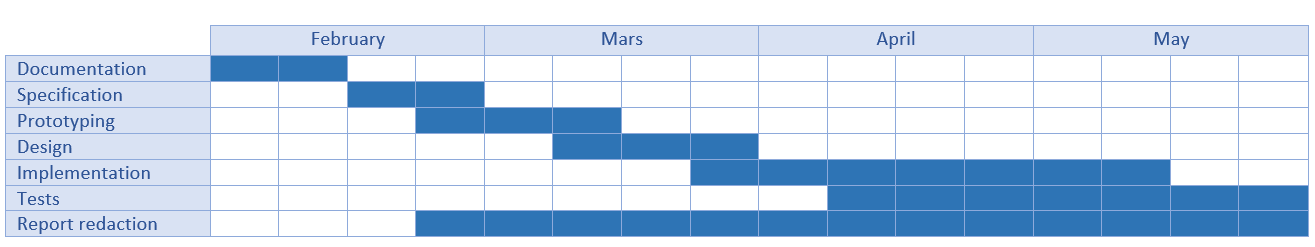
\includegraphics[width=17cm,height=5cm]{Plan.png}
\end{center}
%légende de l'image

\end{table}
\chapter{Conclusion}
Through this software requirements specification we tried to present a reference for the next steps
during the project’s development process. Considering the work progress, we will do our best to be
faithful to the specification characterized above.
%\chapter*{Introduction générale} % Pas de numérotation
\addcontentsline{toc}{chapter}{Introduction générale}


Depuis l’invention du premier avion en 1903 appelé Wright Flyer, la gestion de trafic aérien fut un des défis les plus difficiles à résoudre vu le nombre des vols ascendants. Cette gestion a pour but de maintenir en sécurité le trafic aérien, d’ou l’apparition des organismes internationaux qui s’occupent de cette tâche. L’OACI, Office d’Aviation Civile International est l’organisme qui se charge d’établir les protocoles standardisés de de communication entre les différents aérodromes partout dans le monde. Il normalise aussi les types de messages échangés ainsi que les canaux de transfert utilisés. L’OACA, Office des Aéroport et d’Aviation Civile, qui dérive de l’OACI, est l’organisme nationale qui s’occupe de l’espace aérien tunisien. Sa tâche est de s'occuper de tout ce qui est en relation avec les aéroports internationaux existants sur le territoire tunisien. Cet organisme est décomposé en plusieurs divisions, parmi lesquelles on cite; le centre de contrôle régional. \\

Dans le domaine du contrôle aérien, un centre de contrôle régional, est un centre assurant la sécurité du trafic aérien. L’échange de messages aéronautiques entre ces centres assure l’exécution sûre, rapide et efficace des vols. Il consiste aussi à accélérer et ordonner la circulation aérienne. C’est pour cela que la disponibilité des liaisons entre ces centres s’avère indispensable décisif vu son importance dans la sécurité de la navigation aérienne, la régularité des vols, et le traitement des messages aéronautiques. \\

La diponibilité des messages aéronautiques est un affaire indispensable. Dans ce cadre, s'inscrit notre projet de stage d'immersion en entreprise qui a pour but la conception et la réalisation d'une solution d'apurement de la base de données du système STANOS.\\

Le présent rapport s'organise autour de cinq chapitres:\\
Le premier chapitre intitulé {\bf "Présentation générale"} comprend une présentation de l'organisme dans lequel nous avons effectué notre stage. Il comprend aussi une définition du système autour duquel se déroule notre stage. \\
Le deuxième chapitre intitulé {\bf "Étude préalable"} comprend une revue théorique des notions sur lesquelles s’appuie notre projet en une étude de l’existant, des critiques et une proposition solution à notre problématique.\\
Le troisième chapitre intitulé  {\bf "Analyse et spécification des besoins"} expose la spécification des besoins fonctionnels et non fonctionnels de l’application.\\
Un quatrième chapitre intitulé  {\bf "Conception"} met en évidence la modélisation conceptuelle de l’application.\\
Le dernier chapitre intitulé  {\bf "Réalisation"} inclut une présentation de l’environnement de travail avec la description de quelques interfaces de l’application.\\

Enfin, nous clôturons ce rapport par une conclusion générale dans laquelle nous résumons notre solution et exposons quelques perspectives futures.\\

%\chapter{Présentation générale}

Dans ce premier chapitre, nous commençons par présenter brièvement l'organisme d'accueil au sein duquel nous avons effectué le stage relatif au présent projet. La suite du chapitre est consacrée à présenter le projet autour duquel se déroule notre stage.
%note en bas de page
\section{Présentation de l’organisme d’accueil }

Dans cette partie, nous allons présenter l'Office de l'Aviation Civile et des Aéroports, l'organisme au sein duquel nous avons effectué notre stage. 
\subsection{Présentation de l’OACA}

L’Office de l’Aviation Civile et des Aéroports (OACA) est un établissement public à caractère industriel et commercial doté de la personnalité civile et de l'autonomie financière. Il était créé en 1971, et il est initialement nommé l’Office des Ports Aériens de Tunisie (OPAT). Il est sous tutelle du Ministère du Transport et est chargé de gérer, de développer et d'exploiter les Aéroports Internationaux de la Tunisie (Tunis-Carthage, Enfidha-Hammamet, Monastir Habib Bourguiba, Djerba-Zarzis, Tozeur-Nafta, Sfax-Thyna, Tabarka-AinDraham, Gafsa-Ksar et Gabès-Matmata).\\


\begin{figure}[!h]
\begin{center}
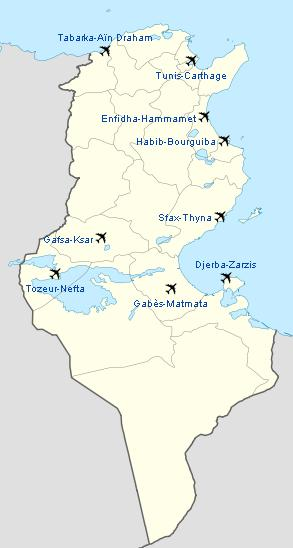
\includegraphics[width=6cm,height=8cm]{presentation/pres1.jpg}
\end{center}
%légende de l'image
\caption{Les divers aérodromes dans le FIR tunisien}
\end{figure}

L'office de l'aviation civile et des aéroports est chargé notamment des missions suivantes:\\
\begin{itemize}
\item L'exploitation, l'aménagement et le développement des aéroports ainsi que l'accomplissement de toutes les opérations et services nécessaires aux voyageurs, aux aéronefs, au fret et au courrier aérien dans les aéroports, \\
\item Le contrôle régional, la gestion de la navigation aérienne et la participation à l'exécution des plans de recherches et de sauvetages, \\
\item La délivrance de tous les documents requis pour le personnel aéronautique, les aéronefs et la navigation aérienne conformément à la législation en vigueur, \\
\item Accomplir la mission du contrôle de la navigation aérienne conformément aux normes internationales en assurant la sécurité, la régularité et la  Fluidité du trafic requis, \\
\item Maintenir aux plus hauts niveaux la sûreté et la sécurité des aéroports conformément aux dispositions internationales, \\
\item Veiller à l'adaptation des installations et des infrastructures aéroportuaires au besoin du trafic aérien, \\
\item Assurer la sécurité et la régularité du trafic en route dans les limites de l'espace aérien. \\
Pour faire à ces obligations internationales et assurer ses responsabilités dans le domaine de la sécurité aéronautique, un centre de navigation aérienne a été implanté par l'OACA. \\
\end{itemize}
\subsection{Organigramme de la Direction des Equipements de la Navigation Aérienne}

La direction des équipements de la navigation aérienne regroupe quatre divisions:\\
\begin{itemize}
\item Division Radar, \\
\item Division Etude et Coordination,\\
\item Division Equipements Aides à la Navigation Aérienne,\\
\item Division Télécommunication Aéronautique (Unité d’accueil).
\end{itemize}
\begin{figure}[!h]
\begin{center}
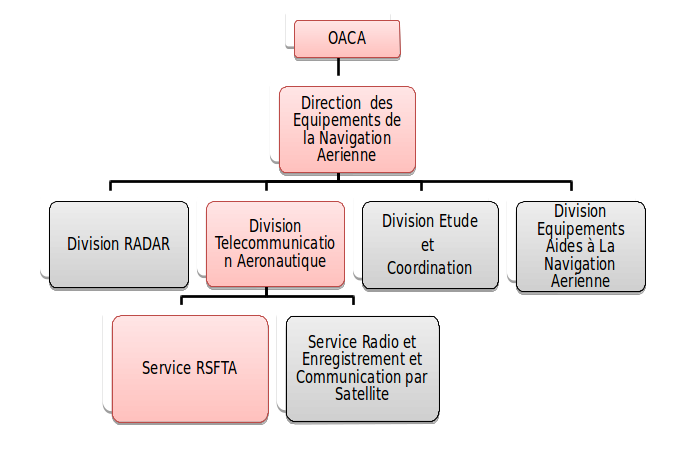
\includegraphics[width=15cm,height=6cm]{presentation/organisme.png}
\end{center}
\caption{Organigramme de la Direction des Equipements de la Navigation Aérienne}
\end{figure}
\subsection{Activités internationales}
Sur le plan international, l’Office de l’Aviation Civile et des Aéroports (OACA) occupe une place de plus en plus importante au sein des instances arabes, africaines et mondiales telles que le Conseil de l’Aviation Civile des Pays Arabes (A.C.A.C), la Commission Africaine de l’Aviation Civile (C.A.F.A.C), l’Organisation de l’Aviation Civile Internationale (O.A.C.I), le Conseil International des Aéroports (A.C.I)… \\

L’O.A.C.A est membre du Conseil International des Aéroports Région Afrique et préside le Groupe Régional de Planification et de Mise en Oeuvre de Plan de Navigation Aérienne pour l’Afrique et l’Océan Indien (A.P.I.R.G). Il est également membre du Conseil d’Administration du Fonds A.C.I.\\

L’Office s’est distingué ces dernières années par la qualité de l’organisation, en Tunisie, de manifestations et de conférences de taille se rapportant aux domaines de l’aviation civile, la gestion et la sûreté aéroportuaire.\\

L’O.A.C.A a également signé des conventions de partenariat avec son homologue au Maroc (O.N.D.A), la Société des Aéroports en Mauritanie (S.M.A), la Société des Aéroports de Paris (A.D.P) et l’Aéroport de Nice Côte d’Azur.\\

L'O.A.C.A emploie des compétences souvent sollicitées pour des travaux d’assistance et d’échange d’expérience avec d’autres pays de notre continent.\\

Les associations et les structures qui évoluent au sein de l’O.A.C.A, telles que l'Association Tunisienne des Contrôleurs de la Circulation Aérienne (A.T.C.C.A), l'Association des Electroniciens de la Sécurité Aérienne (A.T.E.N.A), l'Association des retraités de l'Office, l'amicale du personnel ainsi que l'Association Sportive (A.S.A.C.A), contribuent à renforcer le rayonnement de l'Office à l'échelle internationale par la participation de ces associations et structures à ce niveau à des activités diverses sportives, techniques, sociales….\\

\subsection{Service Réseau de Services Fixes de Télécommunications Aéronautiques}

Le service RSFTA  relève de la Direction des équipements de la navigation aérienne du Centre de Contrôle Régional. Elle  opère avec le Bureau Central des Télécommunications Aéronautiques qui est aussi le centre COM principal de Tunis et fonctionne en étroite collaboration avec le Service d’Information Aéronautique. Elle est chargée de la gestion, l’exploitation et la supervision du système autocommutateurs des messages aéronautiques (ADAMS) qui constitue une composante primordial du Réseau des services Fixes des Télécommunications Aéronautiques (RSFTA). \\

N’importe quel pays dont l'espace aérien sera traversé par le vol est dit pays partageant  ce vol et le besoin d'échange d'information entre pays qui partagent un vol est primordial.
Cet effort de collaboration fut possible pendant de nombreuses années grâce à l'aide de l’Aeronautical Fixed Telecommunications Network (AFTN) ou (RSFTA) en Français. \\
\section{Présentation du système autocommutateur des messages aéronautiques et du réseau AFTN/AMHS}

\subsection{Présentation du réseau AFTN (RSFTA)}

Le réseau des services fixes de télécommunications aéronautiques (RSFTA)  est un réseau mondial des circuits fixes aéronautiques, destiné dans le cadre du service fixe aéronautique, à l’échange des messages et/ou des données numériques entre les stations fixes aéronautiques ayant des caractéristiques de communications identiques ou compatibles. Ces messages aéronautiques ont essentiellement pour but d’assurer la régularité et la sécurité des vols  dans l’espace aérien tunisien. \\ 

Les différentes Catégories des messages qui sont  acheminées par le réseau du service fixe des télécommunications Aéronautiques sont : \\


\begin{itemize}
\item Messages de détresse. \\
\item Messages d’urgence. \\
\item Messages intéressant la sécurité et la régularité (plan de vols, autorisations de survole….). \\
\item Messages météorologiques (METAR, ….). \\
\item Messages des services d’informations aéronautiques (AIS:Notam, Snowtam,..). \\
\item Messages administratifs aéronautiques. \\
\item Messages de service. \\
\end{itemize}
Au niveau de chaque pays le réseau AFTN gère deux types de clients terminaux: \\

	\begin{itemize}
    \item \textbf{Clients nationaux:} Les différents aéroports nationaux et les différentes organisations de l’aviation civile locales ainsi que tout autre siège local pouvant échanger des messages aéronautiques. \\
    
    \item \textbf{Centres internationaux:} Ils sont formés par les centres adjacents qui constituent des nœuds du réseau AFTN et qui assure la fonction de relais pour la transmission des messages aéronautiques entre les différents pays du réseau mondial, dans le cas de la Tunisie les centres adjacents sont Rome, Alger, Tripoli et le Caire.\\

	\end{itemize}

La Tunisie est considérée comme un centre COM principal, parmi six centres principaux de l’Afrique. \\

\begin{figure}[!h]
\begin{center}
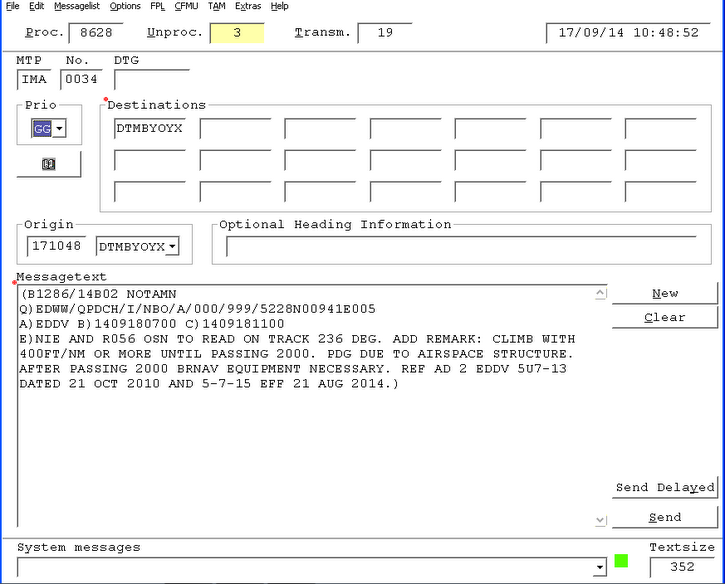
\includegraphics[width=14cm,height=8cm]{presentation/ftn.png}
\end{center}
%légende de l'image
\caption{Exemple de Message AFTN}
\end{figure}
Les champs d’un message AFTN se composent de:\\
\textbf{IMA 0034:} Identification de transmission\\
\textbf{GG:} Indicateur de priorité\\
\textbf{DTMBYOYX:} Indicateur de destinataire \\
\textbf{Origin 171048:} Moment du dépôt (Le groupe date-heure de 6 chiffres précisant le moment auquel le message a été déposé) \\
\textbf{DTMBYOYX:} Indicateur d’origine (identifiant l’expéditeur du message) \\
\textbf{Message Texte:} le contenu du message \\
\subsection{Présentation du Réseau AMHS}

Le réseau AMHS (ATS Message Handling System) est un standard pour la communication  aéronautique sol-sol.Il a été conçu pour remplacer le réseau actuel AFTN vu que ce dernier devenus de plus en plus lourds d’utilisation face à la multiplication importante et active du nombre des intervenants ainsi que l’augmentation considérable, en conséquence, des demandes associées aux services des télécommunications aéronautiques. En effet, en vue d’intégrer le futur réseau mondial de gestion des messages aéronautiques basé sur la technologie IP, pour cela la mise en œuvre de l’AMHS s’est avérée nécessaire. \\

L’avènement de ce nouveau réseau a permis entre autres : \\
\begin{itemize}
\item L’amélioration des services de télécommunications offerts par l’AFTN. \\
\item L’intégration d’autres protocoles de communication tels que le courrier électronique. \\ 
\item L’amélioration de la sécurité du réseau. \\
\item L’interopérabilité avec les autres services de messageries SITA, service militaire, bureau de piste…  \\
\item Le non limitation de longueur ou de type de message avec possibilité d’envoyer des pièces jointes (cartes aéronautiques). \\

\end{itemize}

\section{Présentation du projet}

Dans cette section, le projet sera mis dans son cadre général.\\

\subsection{Cadre du stage}
Ce stage d’immersion en entreprise s’inscrit dans le cadre de formation d’ingénieur en informatique à l’École Nationale des Sciences de l’Informatique (ENSI). Le présent travail se déroule au sein de l’entreprise OACA durant la période entre 01/08/2016 et 09/09/2016.
\subsection{Présentation du sujet}
Il s'agit de l’exécution d’une opération d’apurement pour remédier à la lenteur importante observée au niveau de la production des PIB ainsi que l’élaboration des check-lists. L’apurement des bases de données distantes situées au niveau des différents aéroports a pour objectif de faciliter le travail des exploitants. Notre tâche consiste alors à concevoir une solution pour l'apurement de la base de données de serveur de messages et la développer dans une application.\\
\section*{Conclusion}

Dans ce chapitre nous avons présenté l’entreprise accueillante ainsi que le projet à réaliser et son cadre. Dans le prochain chapitre nous détaillerons quelques concepts en relation avec le sujet afin de mieux
comprendre le déroulement de ce projet.




%\chapter{Étude préalable}

Nous allons exposer tout au long de ce chapitre une synthèse des notions théoriques que nous avons élaboré sur des concepts technologiques qui feront par la suite la base de notre pratique, c'est en effet le contenu de la partie "État de l'art".
À la fin, nous étudions et critiquons des l'existant afin d’introduire notre solution et la positionner par rapport à ce qui existe déjà. \\

\section{État de l'art}
Dans cette section, nous nous intéressons à présenter les deux systèmes utilisés pour la communication des sites aériens; ADAMS et STANOS, tout en définissant leurs compositions et leurs architectures. 
\subsection{Présentation générale du système ADAMS}
\subsubsection{Contexte général}
Le système ADAMS  (Aeronautical Data And Message Handling System) est le système autocommutateur des messages aéronautiques, mis en service en Tunisie depuis l’année 2008  pour l’enregistrement, le traitement et l’acheminement des messages aéronautiques. \\

Il est doté de fonctions et d’outils de contrôle et de supervision permettant d’assurer le bon fonctionnement  des processus de traitement des messages aéronautiques sur le réseau AFTN/AMHS conformément aux recommandations de l’Organisation de l’Aviation Civile Internationale OACI.

\subsubsection{Supervision et exploitation du système}

Le système ADAMS est supervisé 24H par des opérateurs qui assurent le contrôle des différentes opérations et actions se rattachant au système ainsi que la supervision de l’état du réseau d’exploitation sur lequel il opère. Cette supervision continue du système est réalisée  via un système approprié de commandes.\\

Les superviseurs exécuteront leurs tâches quotidiennes sur le système ADAMS à travers les positions MCP (position de contrôle et de supervision des messages et des liaisons) qui sont des stations de supervision connectées directement au central via le réseau LAN, cette tâche consiste à: \\
\begin{itemize}
\item Envoyer et recevoir des messages de formats AFTN ou AMHS.\\
\item Recevoir des messages de format SITA.\\
\item Superviser les différentes activités d’acheminement.\\
\item Vérifier l’état des lignes et circuits.\\
\item Prendre connaissance de l’état opérationnel du centre.\\
\item Suivre les différentes opérations techniques du système.\\
\end{itemize}

\subsubsection{Système de gestion ADAMS}
Le système de gestion ADAMS est un module logistique responsable de la fourniture des outils de gestion de l’interface Homme Machine via laquelle l’opérateur peut inter réagir avec les différentes fonctionnalités du système et de contrôler, superviser et gérer les différents mécanismes logiciels disponibles pour  mener  à bien le processus d’acheminement des, messages aéronautiques, assurer le fonctionnement correct de la partie matérielle du système et garantir la disponibilité optimal du réseau d’exploitation.

\subparagraph{Système de gestion de l’acheminement des messages sous ADAMS:}

Ce module permet au système ADAMS de supporter les différentes technologies de télécommunications avancées par l’OACI telles que l’AFTN et l’AMHS. En effet via ce module de gestion de l’acheminement des messages sous ADAMS, le centre COM principal de Tunis peut être, à la fois, vu comme étant: \\
\begin{itemize}
\item Un centre AFTN. \\
\item Un «Gateway» AMHS / AFTN. \\
\end{itemize}

\subsubsection{Composition d’ADAMS:}
~~\\ 
~~\\
\textbf{- Deux serveurs:} un serveur de secours et un autre opérationnel. On trouve dans chacun, des disques durs de grandes capacités gérés par un système d’exploitation (linux).\\

\textbf{- Deux MSA (Modular Smart Array):} c’est un équipement composé de plusieurs disques sur lesquels est stockée la base de données du système     ADAMS. On  a un MSA fonctionnel et un autre de secours. Chaque MSA contient 5 disques durs (4 fonctionnels et 1 de secours). On peut aussi ajouter des extensions. Au dessus de chaque MSA on trouve un écran digital qui indique l’état de l’ MSA. \\

\textbf{- Deux routeurs:}  routeur est un dispositif situé en un nœud d'un réseau de données qui détermine, pour chaque trame, paquet ou cellule, la route à suivre dans le réseau. \\

\textbf{- Modem:}  Le modem est un dispositif permettent à deux terminaux (console PC) de communiquer à travers une ligne de télécommunication (ligne téléphonique). Les données des terminaux sont transformées par le modem en signaux électriques  de nature acceptable par le réseau de télécommunication, cette transformation est la modulation et démodulation. \\


\textbf{- Switch (A/B):} (AUTOMATIC SWITCHING SYSTEM) c’est un équipement de commutation automatique à large étendue d’applications. Il permet dans notre cas la commutation entre un équipement principal et un équipement de secours assurant ainsi la disponibilité du système. \\


\textbf{- Deux firewalls:} c’est un élément du réseau, qui a pour fonction de faire respecter la politique de sécurité du réseau. Il est généralement installé dans le réseau local de l’entreprise et permet principalement la protection des ressources (serveurs de fichiers, de messagerie, base de données …etc.) des attaques et des accès interdits.\\ 


\subsubsection{Architecture matérielle du système ADAMS}
Le système central ADAMS se compose de:\\ 
\begin{itemize}
\item ne partie serveur autocommutateur de messages AFTN/AMHS  qui contient deux serveurs HP ProLiant DL380 Génération 7 et un système de stockage externe MSA d2000 formant ensemble un système de cluster. Cette partie serveur effectue, lors de la réception d’un message le traitement, l’acheminement et le stockage des messages aéronautiques dans une base de données. \\
\item Une partie réseau qui assure la liaison du cluster avec les différents clients en utilisant les technologies de communications LAN/WAN, Ligne Spécialisée, liaison satellitaire, RTC, FRAME RELAY et RNIS et les protocoles de communications V24 et TCP/IP. \\
\end{itemize}
\begin{figure}[!h]
\begin{center}
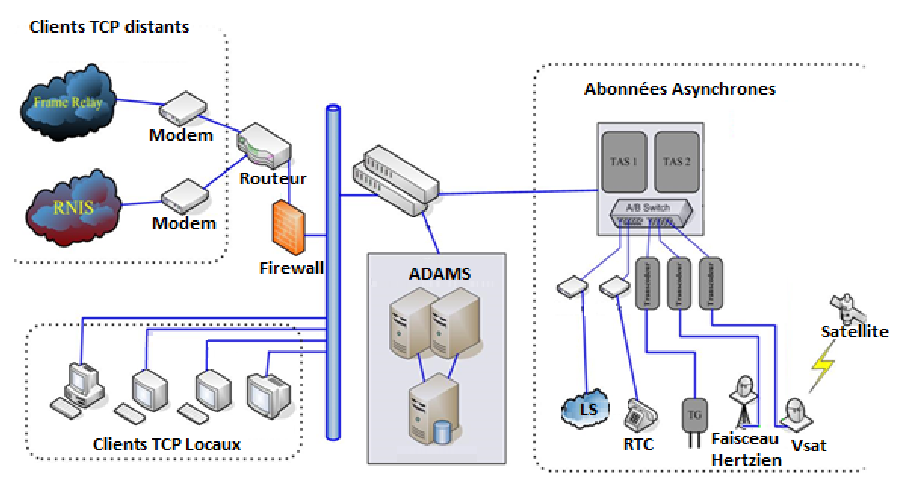
\includegraphics[width=13cm,height=5cm]{existant/architecture.png}
\end{center}
%légende de l'image
\caption{Autocommutateur de message RSFTA}
\end{figure}



\subsection{Présentation générale du système STANOS}
\subsubsection{Contexte général}
A fin d’améliorer sa qualité de service et suivre l’évolution technologique, l’OACA (Office de l’Aviation Civile et des Aéroports) a procédé à l’automatisation du processus d’émission et de réception des messages aéronautiques tels que les \textbf{NOTAM} et \textbf{SNOWTAM}. En effet, l’automatisation de telles tâches peut diminuer le nombre d’erreurs et d’omissions qui peuvent exister au cours de l’exploitation. \\

Par ailleurs, cette tendance d’automatisation des différents processus associés au traitement de l’information aéronautique ne peut être assurée que suite à la création d’une banque de données spécifique de messages aéronautiques regroupant principalement les \textbf{NOTAM} et \textbf{SNOWTAM}. Le logiciel de traitement automatisé des \textbf{NOTAM/SNOWTAM} ou STANOS permet, entre autres, la saisie automatique de ces messages, leur traitement, leur stockage dans la banque de données ainsi que la recherche et la présentation des informations suivant des formats spécifiques tout en satisfaisant un ou plusieurs critères bien déterminés.\\

Le système offre notamment les fonctions suivantes: \\
\begin{itemize}
\item Réception des messages RSFTA (Réseau des Services Fixes des Télécommunications Aéronautiques) à travers les deux liaisons CNA STANOS A et CNA STANOS B reliant le BNI avec le système central d’acheminement des messages aéronautiques ADAMS. \\
\item Validation de tous les NOTAM/SNOWTAM.\\
\item Archivage des NOTAM/SNOWTAM. \\
\item Distribution des NOTAM/SNOWTAM. \\
\item Traitement des messages rejetés. \\
\item Production des bulletins d’information pré-vol PIB en réponse à des requêtes de PIB bien déterminées. \\
\item Diffusion de récapitulatifs de résumés des NOTAM figurant dans la banque de données. \\
\item Création et modification des données géographiques.
\end{itemize}
\subsubsection{Architecture du système STANOS}
\paragraph{Architecture de la base de données STANOS}
~~\\

Le système STANOS est composé d’un ensemble d’applications qui fonctionnent autour d’une base de données distribuée sur plusieurs sites distants. Son fonctionnement est, par conséquent, basé sur une architecture réseau ‘client-serveur’ dont la partie serveur est installée au niveau du Bureau NOTAM International BNI du service de l’Information Aéronautique SIA de la direction de la Navigation Aérienne.\\

La partie serveur comporte des applications spécifiques ainsi qu’une base de données centrale, cette base contient tous les messages aéronautiques NOTAM transmis vers la Tunisie, ces données seront archivés pour des raisons de sécurité de la navigation aérienne (besoins d’enquêtes, traçabilité etc.), tandis que les parties clientes sont installées au niveau des Bureaux d’Information Aéronautique BIA des différents aéroports internationaux tunisiens.\\

Par ailleurs, un module de Distribution sert à alimenter les bases de données locales installées aux niveaux des différents Bureaux d’Information Aéronautique BIA.
~~\\
\begin{figure}[!h]
\begin{center}
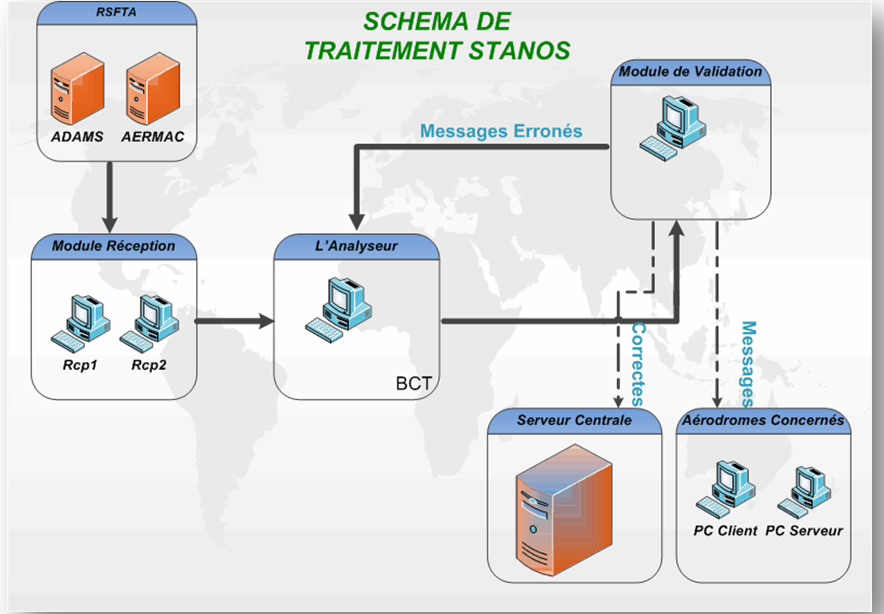
\includegraphics[width=17cm,height=10cm]{existant/architecturestanos.png}
\end{center}
%légende de l'image
\caption{Architecture de la base de données STANOS}
\end{figure}
\newpage
\paragraph{Architecture réseau}
~~\\

Le système STANOS assure la liaison et la distribution des messages aéronautiques NOTAM vers ses clients qui sont les aéroports de la Tunisie: Aéroport International Tunis Carthage, Aéroport International Enfidha Hammamet, Aéroport International Monastir Habib Bourguiba, Aéroport International Djerba Zarzis, Aéroport International Sfax Tina, Aéroport International Tozeur Nefta, Aéroport International Gafsa Ksar, Aéroport International Tabarka Ain Draham.\\

Tous les aéroports sont liés via la liaison Frame Relay sauf l’AITC qui est situé sur le réseau Local du système Central, il est interconnecté via  une liaison fibre optique.   

\begin{figure}[!h]
\begin{center}
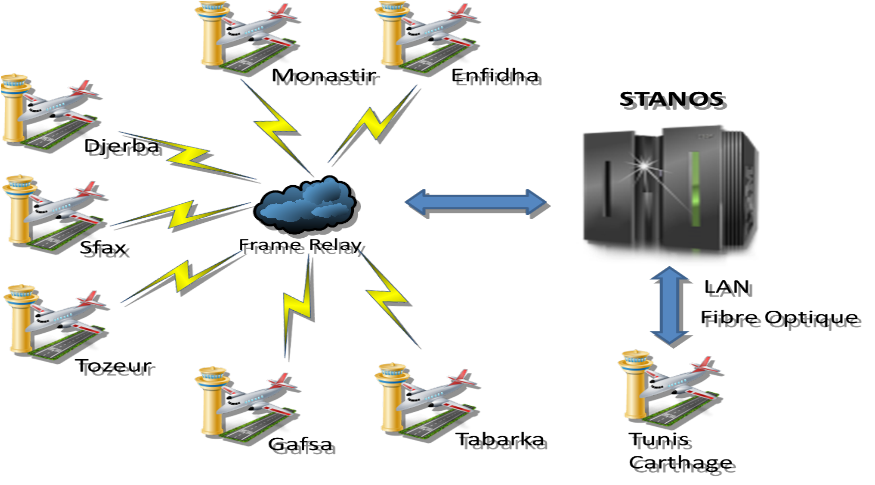
\includegraphics[width=13cm,height=7cm]{existant/stanos.png}
\end{center}
%légende de l'image
\caption{schéma général des liaisons réseaux}
\end{figure}

\begin{figure}[!h]
\begin{center}
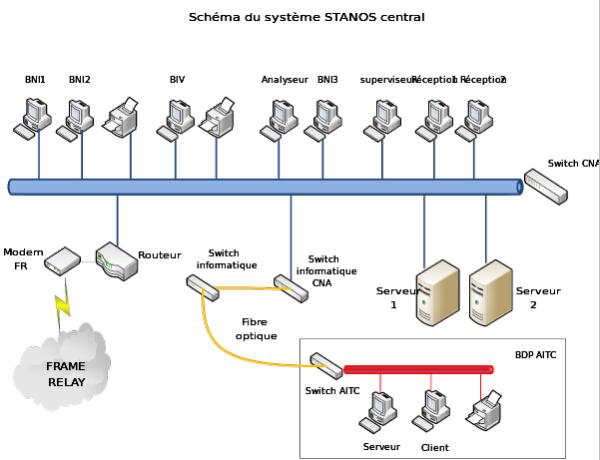
\includegraphics[width=13cm,height=7cm]{existant/Untitled.png}
\end{center}
%légende de l'image
\caption{Architecture centrale du système STANOS}
\end{figure}
\newpage
\paragraph{Fonctionnement global}
~~\\

Dès leur réception sur les lignes RSFTA reliant le Bureau Notam International BNI du service d’Information Aéronautique SIA au système automatique central d’acheminement des messages aéronautiques ADAMS, le système STANOS assure leur traitement immédiat. Ces messages sont ensuite tracés, analysés, validés et enregistrés, au niveau de la base de données centrale du BNI, sous forme d’informations exploitables par les agents d’exploitation de la navigation aérienne  autorisés à cet effet.\\

Le module de distribution ,quant à lui, commence par détecter les nouveaux messages introduits dans la base de données centrale puis analyse sa zone de couverture pour enfin les distribuer vers le ou les Bureaux d’Information Aéronautique concernés au niveau des aéroports internationaux tunisiens. Ainsi, chaque BIA aura une image réduite de la base de données centrale.\\

D’un autre côté, il est à noter qu’au niveau du BIA, l’opération de validation se limite à mettre les messages reçus en zone ou hors zone. Toutes les opérations de traitement (Analyse, correction et validation) se font, de façon centrale, au niveau du BNI.\\


\begin{figure}[!h]
\begin{center}
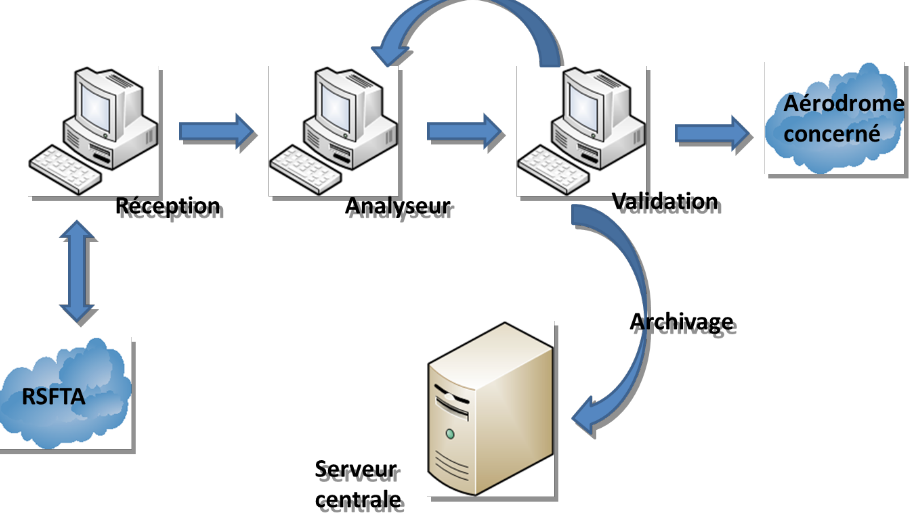
\includegraphics[width=11cm,height=5cm]{existant/fnc.png}
\end{center}
%légende de l'image
\caption{Fonctionnement du système STANOS}
\end{figure}

\section{Etude de l'éxistant}
Le Système autocommutateur de messages aéronautiques assure l’acheminement des messages via deux types de liaisons:\\
\begin{itemize}
\item Liaison synchrone\\
\item Liaison asynchrone\\
\end{itemize}

\subsection{Liaison Synchrône}

Les liaisons synchrones sont utilisées uniquement pour reliés les clients AFTN nationaux.\\
\begin{figure}[!h]
\begin{center}
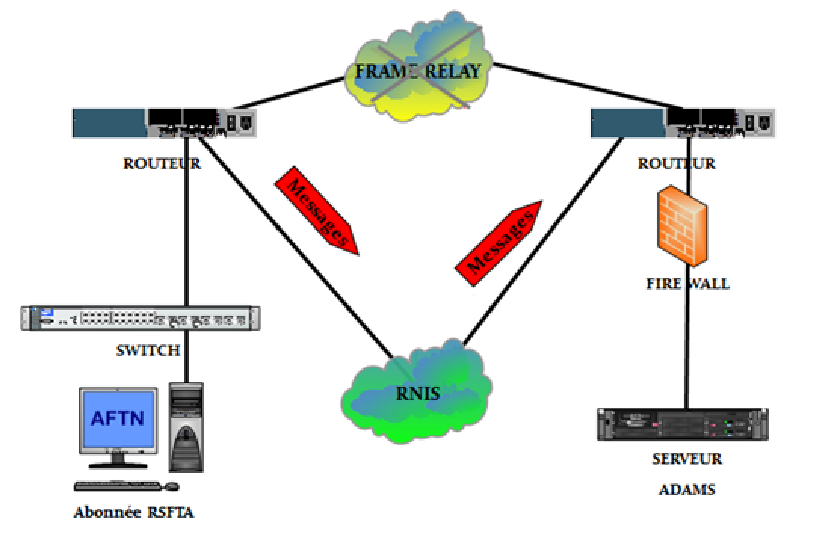
\includegraphics[width=15cm,height=7cm]{existant/sync.png}
\end{center}
%légende de l'image
\caption{Support d’acheminement synchrône}
\end{figure}
 \subsubsection{Frame Relay (Support principal)}
 
 Le Frame Relay est utilisé comme un support de transmission principale pour les échanges entre les différents aéroports. Il établit, en mode connecté, une liaison virtuelle entre les deux extrémités. Cette liaison est permanente (PVC : Permanent Virtual Circuit).\\
 \subsubsection{RNIS (Support de secours)}
 
 Un réseau numérique à intégration de services (RNIS, en anglais ISDN Integrated Services Digital Network) est destiné à remplacer le Frame Relay en cas de panne.\\
Il est caractérisé par :\\
\begin{itemize}
\item Etablissement très court de la communication.\\
\item Débit garanti à 64Kbits/s (et jusqu'à 2Mbits/s).\\
\item Taux d’erreur très faible.\\
\item Cout sur temps de communication.\\
\end{itemize}
\subsection{Liaison asynchrone}

Les liaisons asynchrones sont utilisées  pour acheminer les messages vers les clients nationaux en tant que support de transmission secours en cas de coupure des liaisons synchrones. Seules les abonnées internationales utilisent ces liaisons asynchrones comme des liaisons principales non secourues. \\

\begin{figure}[!h]
\begin{center}
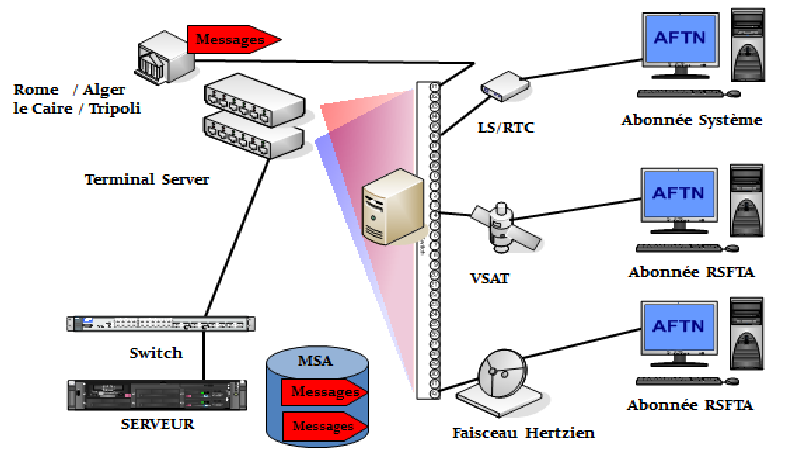
\includegraphics[width=14cm,height=7cm]{existant/asyn.png}
\end{center}
%légende de l'image
\caption{Supports d’acheminement Asynchrone}
\end{figure}
\subsubsection{Faisceau Hertzien}

Le faisceau hertzien est utilisé pour l’acheminement des messages entre le centre de contrôle régional et l’aéroport internationale Habib Bourguiba ainsi que l’aéroport international Enfidha-Hammamet.\\

Un faisceau hertzien est un système de transmission de signaux  entre deux points fixes. Il utilise comme support les ondes radioélectriques, avec des fréquences porteuses de 1 GHz à 40 GHz, très fortement concentrées à l'aide d'antennes directives. Ces ondes sont principalement sensibles aux masquages (relief, végétation, bâtiments…), aux précipitations, aux conditions de réfractivité de l'atmosphère et présentent une sensibilité assez forte aux phénomènes de réflexion\cite{cite4}. \\

\subsubsection{Satellite}

a liaison satellitaire est utilisée pour l’acheminement des messages entre le centre de contrôle régional et l’aéroport international Djerba-Zarzis ainsi que l’aéroport international Sfax-Tina. \\
VSAT est l'abréviation de Very Small Aperture Terminal. Il désigne un terminal terrestre utilisé au sein d'une communication aérienne par satellite pour l'émission/réception de signaux de données. Il s'agit d'une connexion de données haut débit et illimitée.
Un système VSAT consiste en deux parties : une antenne émettrice/réceptrice placée à l'extérieur du centre de contrôle régional pointant vers le satellite de communications, et un dispositif placé à l'intérieur des aéroports distants.\\

\begin{figure}[!h]
\begin{center}
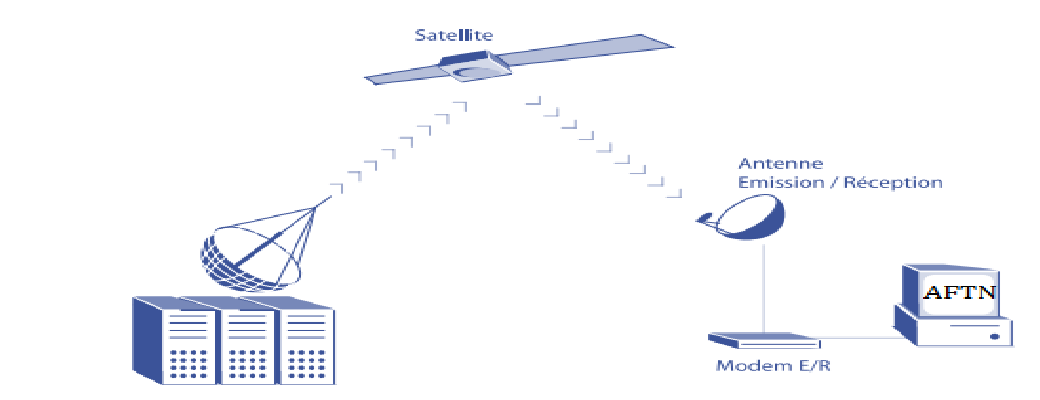
\includegraphics[width=14cm,height=7cm]{existant/sate.png}
\end{center}
%légende de l'image
\caption{Liaison satellitaire}
\end{figure}
~~\\
\subsubsection{RTC (Réseau Téléphonique Commuté)}

La liaison RTC est utilisée pour l’acheminement des messages entre le centre de contrôle régional et l’aéroport international Tabarka-Ain Drahem.\\
Le réseau téléphonique commuté est le réseau du téléphone (fixe et mobile), dans lequel un poste d'abonné est relié à un central téléphonique par une paire de fils. Les centraux sont eux-mêmes reliés entre eux par des liens offrant un débit allant jusqu’à 2 Mb/s Pour établir la communication point à point, l’aéroport AITA et le centre de contrôle régional sont relié à travers deux modems.\\

\subsection{Lignes spécialisées}

Leslignes spécialisées(LS) appelée égalementliaison louée est entélécommunicationune liaison physique de niveau 2, connectée en permanence entre le centre de contrôle régionale de la Tunisie et les autres abonnées internationaux. Elle estmise en œuvreet exploitée par unopérateur de télécommunication sur des longues distances.\\
En réalité la ligne spécialisée n'est souvent dédiée que pour  le site du client et le point d'accès au réseau de l’opérateur de télécommunication.Les données étant transportées ensuite sur des réseaux d'opérateurs de télécommunications, sur lesquels seule la bande passante est dédiée donc elle est onéreuses.\\
\begin{figure}[!h]
\begin{center}
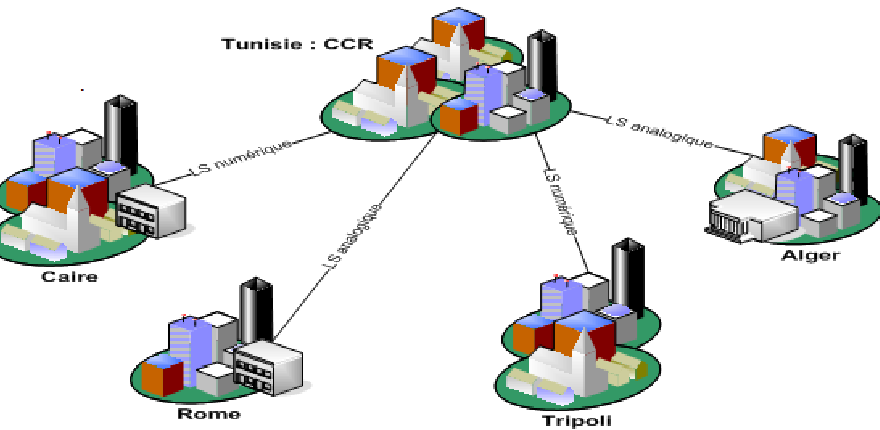
\includegraphics[width=13cm,height=7cm]{existant/ls.png}
\end{center}
%légende de l'image
\caption{Réseau AFTN international}
\end{figure}
\newpage
\subsection{Critique de l'existant}
L’installation du système autocommutateur des messages aéronautiques et du réseau RSFTA/AMHS a bien fonctionné depuis sa mise en marche en 2006. La séparation de traitement des NOTAM des autres messages (les NOTAM sont traités par le STANOS et les autres messages par l’ADAMS) a pour améliorer le temps de réponse et a permis la bonne gestion des messages. Mais après une dizaine d’année d’exploitation, les exploitants de ce système ont remarqué une lenteur importante dans le traitement des messages aéronautiques.  La diagnostique du problème montre que la surcharge du système STANOS par des messages expiré a gravement causé cette lenteur d’où la nécessité d’une opération d’apurement de base de donnée. Pour ne pas tomber dans le même problème prochainement, notre projet de stage consiste à développer une application d’apurement de base de données pour l’utiliser périodiquement dans le but d’assurer le bon fonctionnement de traitement des messages aéronautique.\\
\section*{Conclusion}
Ce chapitre comporte deux sections. La première section intitulée "Etat de l'art" a donné un aperçu sur les deux types de serveurs de messges utilisé au sein de de l'OACA; leurs composition et leurs architectures. La deuxième section a été consacrée à étudier l'exsitant qui nous a aider à révéler leur defaillances et ce afin de déterminer les objectifs et les apports de notre application.
  








%tableau centré à taille variable qui s'ajuste automatiquement suivant la longueur du contenu
% \begin{figure}[!h]
% \begin{center}
% \begin{tabular}{|l|l|l|l|l|}
%   \hline
%   Solution & Critère 1 & Critère 2 & Critère 3 & Critère 4\\
%   \hline
%   Solution 1(cf. ref. \cite{cite0}) & Oui & Oui & Oui & Oui \\
%   Solution 2(cf. ref. \cite{cite1}) & Oui & Oui & Oui & Non \\
%   Solution 3(cf. ref. \cite{cite2}) & Oui (sauf telle chose) & Non & Non & Oui\\
%   Solution 4(cf. ref. \cite{cite3}) & Oui& Non & Oui & Non\\
%   Solution 5(cf. ref. \cite{cite4}) & Oui (uniquement ceux-ci) & Non & Oui & Non\\
%   \hline
% \end{tabular}
% \end{center}
% \caption{Tableau récapitulatif des solutions}
% \end{figure}

 
%\chapter{Analyse et spécification des besoins}

La phase d’analyse et spécification des besoins présente une étape primordiale dans le cycle de développement d’un projet. En effet, elle permet de mieux comprendre le travail demandé en dégageant les besoins des différents utilisateurs que doit le système accomplir. Pour ce faire, dans le présent chapitre nous allons commencer par l’analyse des besoins en détaillant les besoins fonctionnels et non fonctionnels ensuite nous allons présenter les différents cas d’utilisation de l’application et en enfin nous exposons quelques diagrammes de séquence.

\section{Spécification des besoins}

Tout au long de cette section nous allons identifier les différents acteurs qui interagissent avec le système et nous allons énumérer les besoins fonctionnels ainsi que les besoins non fonctionnels.


\subsection{Les besoins fonctionnels}

Notre application doit offrir aux utilisateurs différentes fonctionnalités selon les privilèges de chacun d’entre eux. Ces besoins peuvent être résumés dans les points suivants: \\
\begin{itemize}
\item \textbf{BF1:} Le système doit permettre la gestion des rôles des différents intervenants dans l’opération d’apurement de la base de données. \\
\item \textbf{BF2:} Le système doit accéder aux champs NOTAM expirés de la base de données pour les faire supprimer.\\
\item \textbf{BF3:} Le système doit assurer que chaque opération effectuée doit être validée par un être supérieur, la validation finale doit être suivie par l’exécution de l’opération.\\
\item \textbf{BF4:} Le système doit assurer que chaque opération effectuée doit être enregistré dans un historique qui garde la nature de l’opération, celui qui l’a lancé et ceux qui l’ont validé.\\
\item \textbf{BF5:} Le système doit permettre à un super-administrateur de gérer la liste des différents utilisateurs ; ajouter un compte utilisateur en précisant son type, modifier un profile utilisateur ou bien le supprimer.\\
\end{itemize}

\subsection{Les besoins non fonctionnels}

En plus des besoins, plusieurs considérations et contraintes additionnelles doivent être prises en compte lors de la mise en place de l’application. Ces besoins peuvent se résumer par ce qui suit.

\subparagraph{Ergonomie et convivialité :} L'application doit présenter une interface claire conviviale et ergonomique.
\subparagraph{Maintenabilité :}Le système devra pouvoir être maintenu par des développeurs qui ne sont pas les développeurs d’origine.
\subparagraph{Vitesse de temps de réponse :}La réponse devra être assez rapide pour éviter d’interrompre le flux de pensée de l’utilisateur.
\subparagraph{Évolutivité :}La modularité et l'extensibilité de l'architecture de l'application en cas d'ajout des nouveaux services
\section{Analyse des besoins}

Pour spécifier de façon formelle les besoins requis par l’application, nous avons opté pour la réalisation du diagramme des cas d’utilisation pour avoir une meilleure compréhension des besoins.

\subsection{Identifaction des acteurs}

Dans cette partie, nous identifions les différents acteurs qui agissent sur notre application. En effet, un acteur est un élément externe, qui peut être un être humain, une machine, ou un autre système, qui interagit avec le système pour avoir un résultat.\\

Après avoir étudié les différentes interactions internes et externes du système nous avons jugé nécessaires les acteurs suivants :\\
\begin{itemize}
\item \textbf{Super-Administrateur:} le super-administrateur est un acteur qualifié d’une autorité principale d’accès. Il joue un rôle capital dans l’assurassions du bon fonctionnement du système. C’est la personne qui prend en charge la gestion des comptes des
utilisateurs ainsi la validation des opérations effectuées sur la base de données.\\
\item \textbf{Administrateur:} l'administrateur est un acteur qualifié d'une autorité moins importante que celle d super-administrateur. Cet acteur est chargé de faire les actions préliminaires de validation. Il suggère au super-administrateur l'ajout des comptes utilisateurs. Pour chaque site, on trouve une personne qui joue le rôle d'un administrateur. \\ 
\item \textbf{Agent: } un agent est un acteur principal en interaction directe avec l’application. Il s'agit de la personne qui manipule la base de données en direct. Il génére les messages. Il y a deux type d'agent: Un agent site centrale situé au niveau l AITC et un agent site distant situé au niveau des site aérien autre que l'AITC.\\

\end{itemize}

\subsection{Diagrammes cas d'utilisation}
Après avoir identifier les différents acteurs de notre système, nous réservons cette section pour illustrer le diagramme de cas d'utilisation pour chaque type d'acteur. \\

\subsubsection{Diagramme cas d'utilisation pour le super administrateur}
La figure ci-dessous illustre le diagramme cas d'utilisation pour un super administrateur. En effet, un super administrateur peut, après avoir s'authentifié, valider les opération requise par un agent, gérer les comptes des exploitant, forcer les opérations d'exception en cas d'urgent, et également communiquer avec les autres exploitants par des messages.
\begin{figure}[!h]
\begin{center}
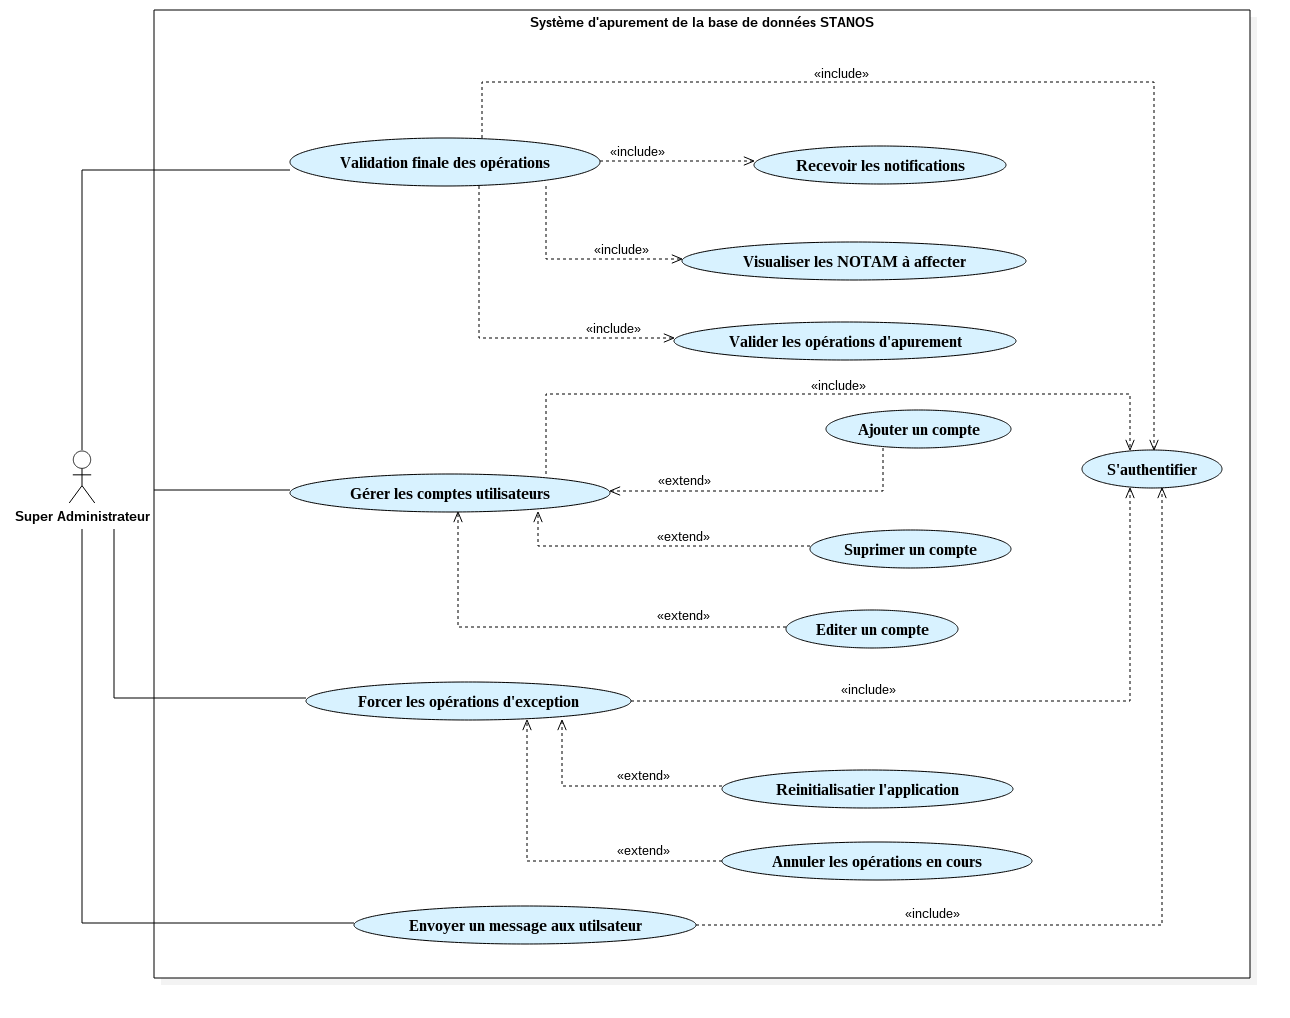
\includegraphics[width=18cm,height=16cm]{besoins/super_administrateur.png}
\end{center}
%légende de l'image
\caption{Diagramme cas d'utilisation pour le super administrateur}
\end{figure}


\subsubsection{Diagramme cas d'utilisation pour l'administrateur}

Le diagramme ci-dessous illustre les cas d’utilisation pour un exploitant de type administrateur. Cet acteur peut effectuer trois différentes actions après avoir s’authentifié. Il valide, alors, d’une manière préliminaire les opérations d’apurement suggéré par l’agent, suggère des modifications sur la liste d’utilisateur et communiquer par messages avec les autres exploitants.\\


\begin{figure}[!h]
\begin{center}
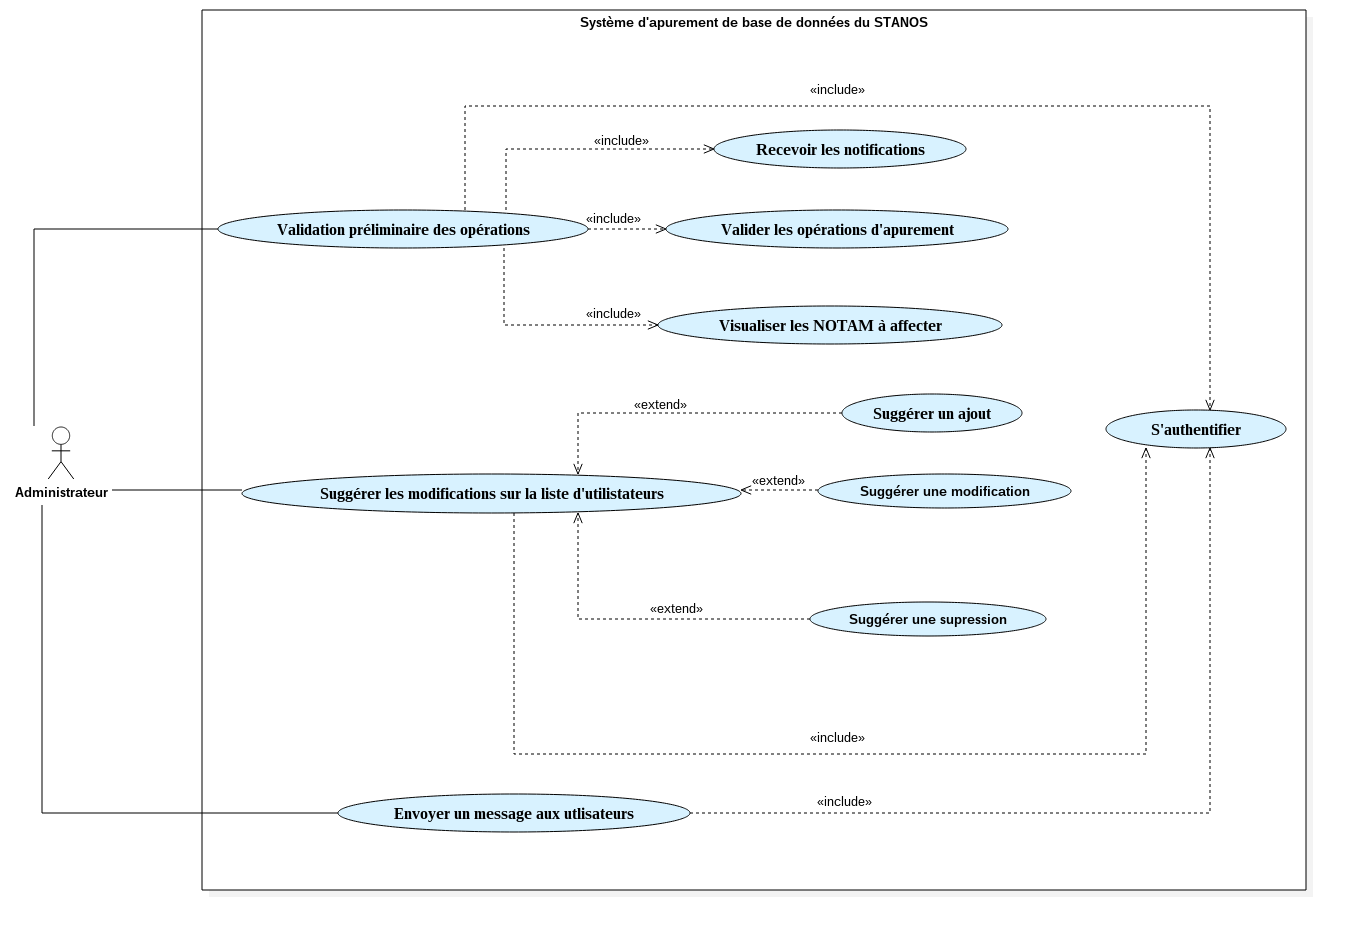
\includegraphics[width=17cm,height=17cm]{besoins/administrateur.png}
\end{center}
%légende de l'image
\caption{Diagramme cas d'utilisation pour l'administrateur}
\end{figure}


\subsubsection{Diagramme cas d'utilisation pour l'agent}

Le diagramme ci-dessous présente les cas d’utilisation pour un agent. Un agent peut effectuer les opérations suivantes après avoir s’authentifié (quoiqu’il soit un agent de site central ou des sites distants) ; lancer des requêtes de mise à jour, valider et tester les lignes sélectionnées et communiquer avec les autres utilisateurs avec messages. Avant de lancer les requêtes d’apurement, un agent site central effectue les opérations suivantes : Création d’un serveur virtuel AIXX, importer la base de AITC vers AIXX et finalement valider les tables NOTAM et PIB. Pour un agent site distant, les opérations à effectuer sont ; sauvegarder une copie de la base existante puis la supprimer, finalement il crée une nouvelle base à partir des lignes validées.

\begin{figure}[!h]
\begin{center}
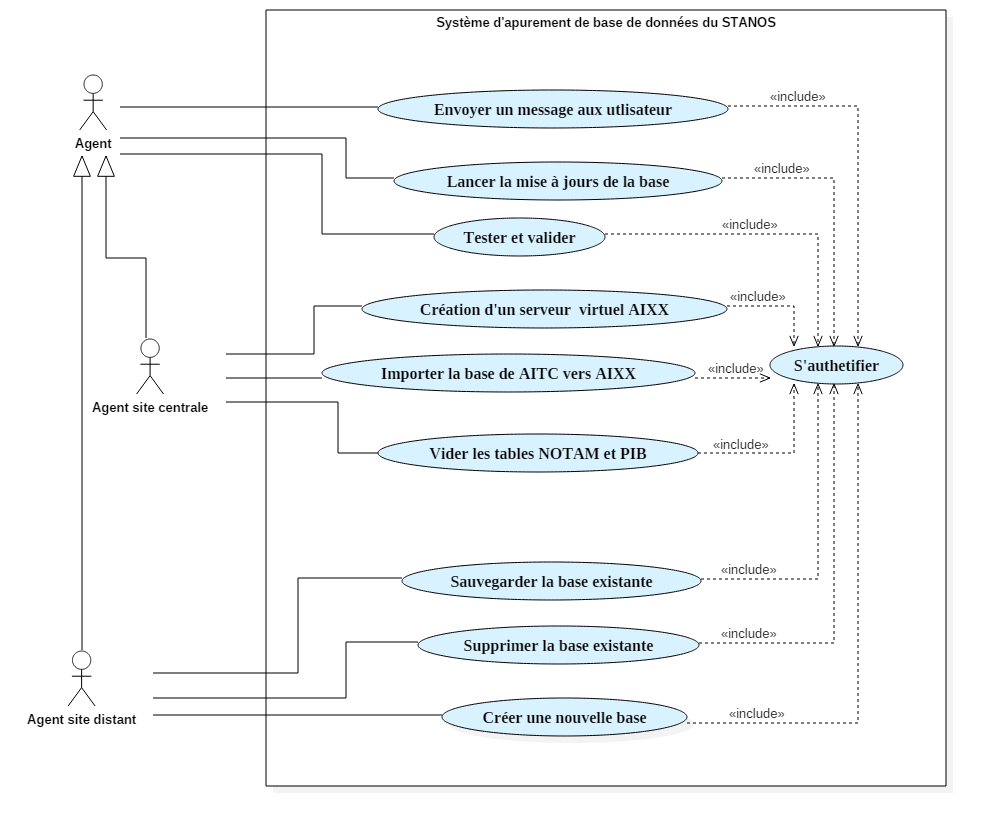
\includegraphics[width=17cm,height=17cm]{besoins/UseCaseDiagram1.png}
\end{center}
%légende de l'image
\caption{Diagramme cas d'utilisation pour l'agent}
\end{figure}
\
\subsection{Diagrammes de séquences système}
Le diagramme de séquence système consiste à décrire l’interaction globale entre le système et l’exploitant. Dans notre système, au premier lieu, l’utilisateur doit fournir séparément un login et un mot de passe pour s’authentifier. Le système vérifie le login et le mot de passe. En cas de correspondance, l’utilisateur est autorisé à accéder aux ressources demandées. Sinon il reste bloqué jusqu’à réussir son authentification.
\begin{figure}[!h]
\begin{center}
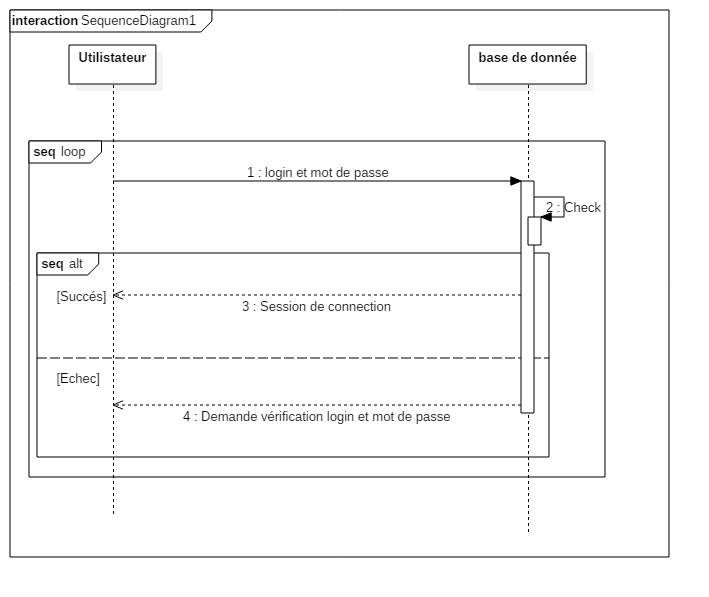
\includegraphics[width=15cm,height=11cm]{Conception/SequenceDiagram2.png}
\end{center}
%légende de l'image
\caption{Diagramme de séquence système}
\end{figure}
\newpage
\subsection*{Conclusion}
Dans ce chapitre nous nous sommes intéressés à l'analyse des besoins fonctionnels et non fonctionnels de notre application. D'autre part, nous avons décelé les cas d'utilisation ainsi que l'acteur principal de l'application et nous avons tracé un diagramme de cas d'utilisation regroupant de manière schématique cette analyse. Enfin, nous avons distingué les différents scénarios qui peuvent avoir lieu, et les dialogues possibles entre le système et le superviseur.











%\chapter{Conception}

La phase de conception est la phase la plus crucial du processus de développement d’une application. En effet, cette phase vise à transformer un concept abstrait en un produit réel. Un projet bien conçu est facile à implémenter et à maintenir. Ainsi, le choix de la conception à adopter est très important afin de mettre au point un système convivial. Ainsi ce chapitre sera consacré à la présentation des différentes étapes de la conception de notre application, et afin de présenter au mieux cette partie nous allons donner une vue globale décrivant le schéma de la solution projetée, la procédure à suivre, l’architecture générale, et la décomposition logique de l’application. Dans une deuxième partie de ce chapitre nous allons utiliser le langage semi-formel UML\cite{cite1} pour illustrer le diagramme de classe et le diagramme entité-relation de la base de données.
\section{Conception générale}
Il est primordiale à la conception de tout système informatique de choisir l’architecture qui lui sera adéquat assurant son bon fonctionnement.

\subsection{Schéma de la solution projetée}
Puisque le système s’exécute sur une architecture réseau bien déterminée et conçu auparavant, on a recours donc à prendre en compte lors de la phase de conception architecture, c’est pourquoi nous proposons une solution qui envoie les requêtes d’apurement sur le réseau existant en mode distribution. L’acheminement des requêtes est présenté par la figure 5.1. 
\begin{figure}[!h]
\begin{center}
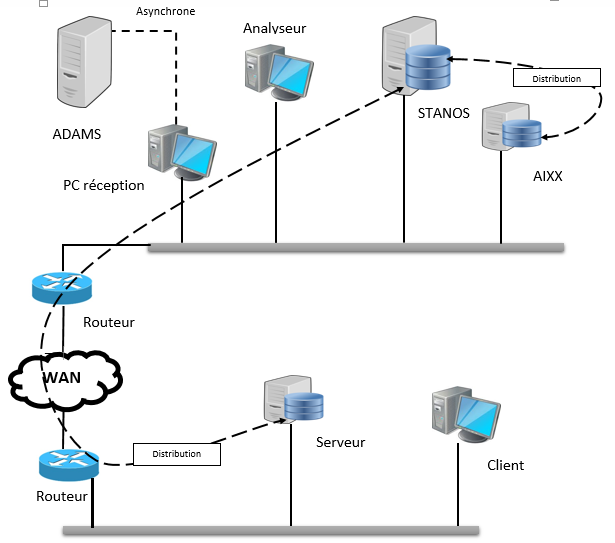
\includegraphics[width=17cm,height=6.5cm]{Conception/solution.png}
\end{center}
%légende de l'image
\caption{Schéma de la solution projetée}
\end{figure}


\subsection{Présentation de la procédure}

\subsubsection{Le site central (CNA)}
\begin{table}[!h]
\begin{center}
\begin{tabularx}{17cm}{|c|p{7.5cm}|X|}
  \hline
  \textbf{Ordre}  & \textbf{Opération à réaliser sur la base virtuelle} & \textbf{Base centrale} \\ \hline
  1 & Création du serveur virtuel AIXX & \\ \hline
  2 & Importer la base AITC ---> AIXX & \\ \hline
  3 & Vider table (NOTAM ...) et (PIB + ...) & \\ \hline
  4 & & Création de l'abonner AIXX + sa zone de couverture \\ \hline
  5 & & Exécusion de la requête SQL de création des lignes de 	distribution des NOTAMs en vigueur de l'abonné AIXX dans la table <<Distribute BNI>> \\ \hline
  6 & Lancement + Mise à jour de la base statique & \\ \hline
  7 & Réindexation & \\ \hline
  8 & Lancement de la distribution & \\ \hline
  9 & Validation & \\ \hline
  10 & Serveur AIXX opérationnel & \\ \hline
  11 & test et vérification : check-list + PIB & \\ \hline

\end{tabularx}
\end{center}
\caption{Tableau des opérations effectuées sur le site central}
\end{table}
\subsubsection{Le site distant(aéroport)}

\begin{table}[!h]
\begin{center}
\begin{tabularx}{17cm}{|c|p{7.5cm}|X|}
  \hline
  \textbf{Ordre} & \textbf{Base distante (Aéroport)} & \textbf{Base centrale} \\ \hline
  1 & Sauvegarder la base existante & \\ \hline
  2 & Supprimer la base existante (Tablespace et user) & \\ \hline
  3 & Création d'une nouvelle base vierge (Tablespace et user) & \\ \hline
  4 & Exporter AIXX crée vers la destination (selon le nom du user) & \\ \hline
  5 & Mettre à jour la table abonnée & \\ \hline
  6 & & Mise à jour la table Distribute-BNI pour redistribuer les données des N jours manquant de trafique de l'abonné \\ \hline
  7 & Lancer les modules BIA et distribution &  \\ \hline
  8 & Mise à jour des données statistique & \\ \hline
  9 & test de validation : check-list et PIB & \\ \hline
  10 & Mise en service & \\ \hline

\end{tabularx}
\end{center}
\caption{Tableau des opérations effectuées sur le site distant}
\end{table}
\newpage
\subsection{Architecture adoptée}
Nous optons pour l’architecture trois-tiers pour la mise en place de notre système. En effet, l’architecture trois-tiers est un modèle logique d’architecture applicative qui vise à séparer très nettement trois couches logicielles au sein d’une même système, à modéliser et à présenter cette application comme un empilement de trois couches. Chaque couche joue un rôle bien précis dans la conception logicielle du système :
\begin{figure}[!h]
\begin{center}
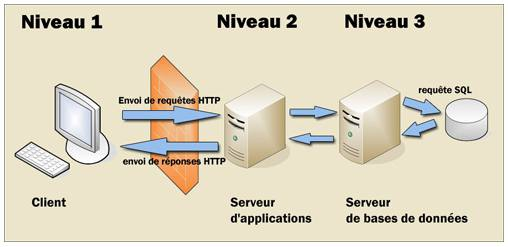
\includegraphics[width=9cm,height=4cm]{Conception/3-tiers.jpeg}
\end{center}
%légende de l'image
\caption{Architecture trois-tiers adoptée}
\end{figure}
\begin{itemize}
{\bf \item La couche présentation :} Elle correspond à la partie de l’application visible et interactive
avec les utilisateurs. On parle d’Interface Homme Machine (IHM). Elle relaie les requêtes
de l’utilisateur à destination de la couche métier, et en retour lui présente les informations
renvoyées par les traitements de cette couche.\\
Dans notre cas la couche présentation correspond à un exploitant de l'application quoiqu'il soit son type, connecté à une session après avoir être s'authentifier. 
{\bf \item La couche métier : }Elle correspond à la partie fonctionnelle de l’application, celle qui implémente
la "logique métier", et qui décrit les opérations que l’application opère sur les
données en fonction des requêtes des utilisateurs, effectuées au travers de la couche présentation.
La couche métier offre des services applicatifs à la couche présentation. Pour
fournir ces services, elle s’appuie, le cas échéant, sur les données du système, accessibles
au travers des services de la couche inférieure. En retour, elle renvoie à la couche présentation
les résultats calculés.\\
Dans notre cas la couche métier correspond au serveur de l'application  qui est chargé de traiter des
requêtes de l'agent envoyées par l’application sous forme de requêtes SQL. 
{\bf \item  La couche accès aux données :} Elle comprend la partie gérant l’accès aux gisements de
données du système. Ces données peuvent être propres au système, ou gérées par un
autre système. La couche métier n’a pas à s’adapter à ces deux cas, ils sont transparents
pour elle, et elle accède aux données de manière uniforme.\\ Dans notre cas, le serveur de base de données (Microsoft SQL Server) permet l'accès aux données stockées dans la base de données non relationnelle.
\end{itemize}
\subsection{Décomposition logique de l’application}
Nous avons utilisé côté client le framework Laravel, c’est un framework basé sur une
architecture MVC\emph ({Modèle/Vue/Contrôleur})\cite{cite3}.\\
En effet Le principe fondamental de ce pattern consiste à distinguer trois entités distinctes qui sont, le modèle, la vue et le contrôleur ayant chacun un rôle précis dans l'interface. 
Dans l'architecture MVC, les rôles des trois entités sont les suivants :

\begin{description}

 {\bf \item Rôle du modèle :}

Le modèle contient les données manipulées par le programme. Il assure la gestion de ces données et garantit leur intégrité. 
Le modèle offre des méthodes pour mettre à jour ces données (insertion suppression, changement de valeur). Il offre aussi des méthodes pour récupérer ces données. Dans le cas de données importantes, le modèle peut autoriser plusieurs vues partielles des données. 

Dans notre application, les modèles vont gérer toutes les données qui se trouvent  dans une base de données.


{\bf \item  Rôle de la vue :}

La vue fait l'interface avec l'utilisateur. Sa première tâche est d'afficher les données qu'elle a récupérées auprès du modèle. Sa seconde tâche est de recevoir toutes les actions de l'utilisateur (clic de souris, sélection d'une entrée, …) . Ces différents événements sont envoyés au contrôleur.

Dans notre application, les vues constituent les pages Web de notre site.


{\bf \item Rôle du contrôleur :}

Le contrôleur est chargé de la synchronisation du modèle et de la vue. Il reçoit tous les événements de l'utilisateur et enclenche les actions à effectuer. 
Si une action nécessite un changement de données, le contrôleur demande la modification des données au modèle et  avertit ensuite la vue que les données ont changé pour que celle-ci se mette à jour.

Dans notre application, le contrôleur va demander au modèle les données, les analyser,  prendre des décisions et renvoyer le texte à afficher à la vue. Ce contrôleur ne contient que du code en PHP et réalise des actions.

\end{description}
\section{Conception détaillée}
Dans cette partie nous allons détailler chaque composant de notre solution, précédemment décrite, d'une façon globale. 
\subsection{Conception de la base de données}
Les tables de la base de données sont les suivantes : \\

\textbf{UTILISATEUR :} c’est la table dans laquelle sont enregistrés tous les utilisateurs de l’application en précisent leurs identifications, leurs appartenances à aérodrome, et leur types.\\

\textbf{TYPE :} c’est la table des différents types des exploitants.\\

\textbf{AERODROME :} c’est la table dans laquelle existent toutes informations sur les aérodromes existant sur le FIR tunisien.\\

\textbf{HISTORIQUE :} cette table a pour but de satisfaire le besoin de sauvegarder l’historique de chaque opération effectuée ; l’agent qui l'a lancé et les administrateurs qui l’ont validé. \\

\textbf{MESSAGE :} pour garder le bon déroulement de l’opération d’apurement de base de données, on a recours à concevoir un modèle de communication entre les différents exploitants du système. Ce modèle est illustré par la table messages.\\

La relation entre ces différentes tables est illustrée par le modèle conceptuel de données suivant : \\

\begin{figure}[!h]
\begin{center}
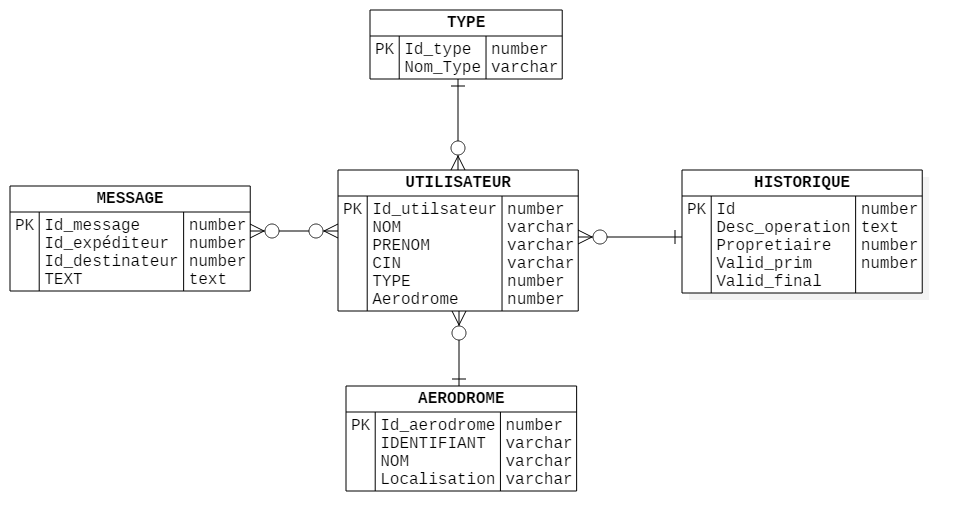
\includegraphics[width=17cm,height=12cm]{Conception/ERDDiagram1.png}
\end{center}
%légende de l'image
\caption{Modèle conceptuel de données }
\end{figure}
\newpage
\subsection{Diagramme de classe}
Notre application, conçue dans une approche orientée objet, donne naissance au diagramme de classes présenté dans la figure 4.4. \\

Une exploitant est modélisé par la classe personne, qui prend comme attribut les identifiant d’une personne. Comme il y a plusieurs types d’exploitant, trois classes hérite de la classe personne, qui sont ; AGENT, ADMINISTRATEUR et SUPER\_ADMINISTRATEUR. Ces trois classe surcharge la méthode ouvrir\_session(). Une personne peut ouvrir une seule session, pour effectuer plusieurs opérations et les inscrire dans un rapport de feedback, d’où la nécessité des classe SESSION, OPERATION et RAPPORT. Seul l’exploitant de type agent est en relation avec les messages aéronautique NOTAM, ceci s’illustre par la relation " consulter " dans le diagramme de classes.\\ 
\begin{figure}[!h]
\begin{center}
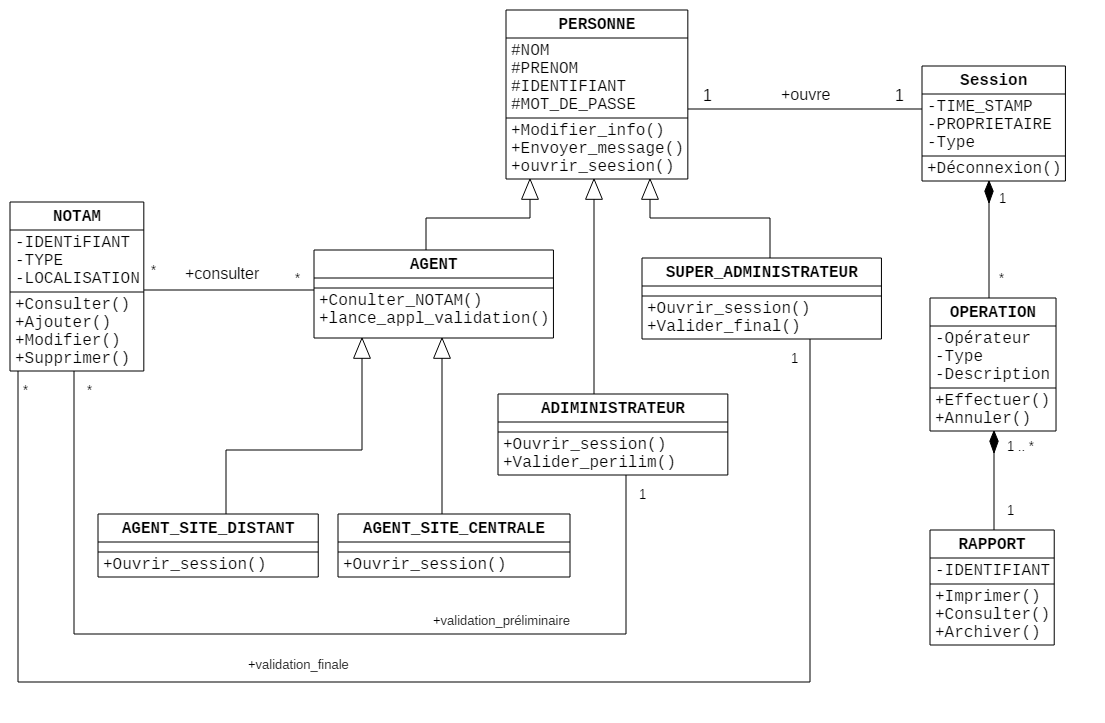
\includegraphics[width=17cm,height=13cm]{Conception/ClassDiagram1.png}
\end{center}
%légende de l'image
\caption{Diagramme de classes}

\end{figure}
\newpage
\subsection{Diagrammes de séquences}
Le déroulement général de l’opération d’apurement s’illustre dans le digramme de séquences ci-dessous, un agent lance une requête d’observation vers la base de données pour sélectionner les lignes de NOTAM à affecter. Après de vérifier, cet agent est appelé à lancer une demande de validation vers l’administrateur. S’il reçoit la validation, il peut lancer alors un bilan de l’opération vers le super-administrateur pour qu’il l’exécute et supprime les lignes expirées.\\
\begin{figure}[!h]
\begin{center}
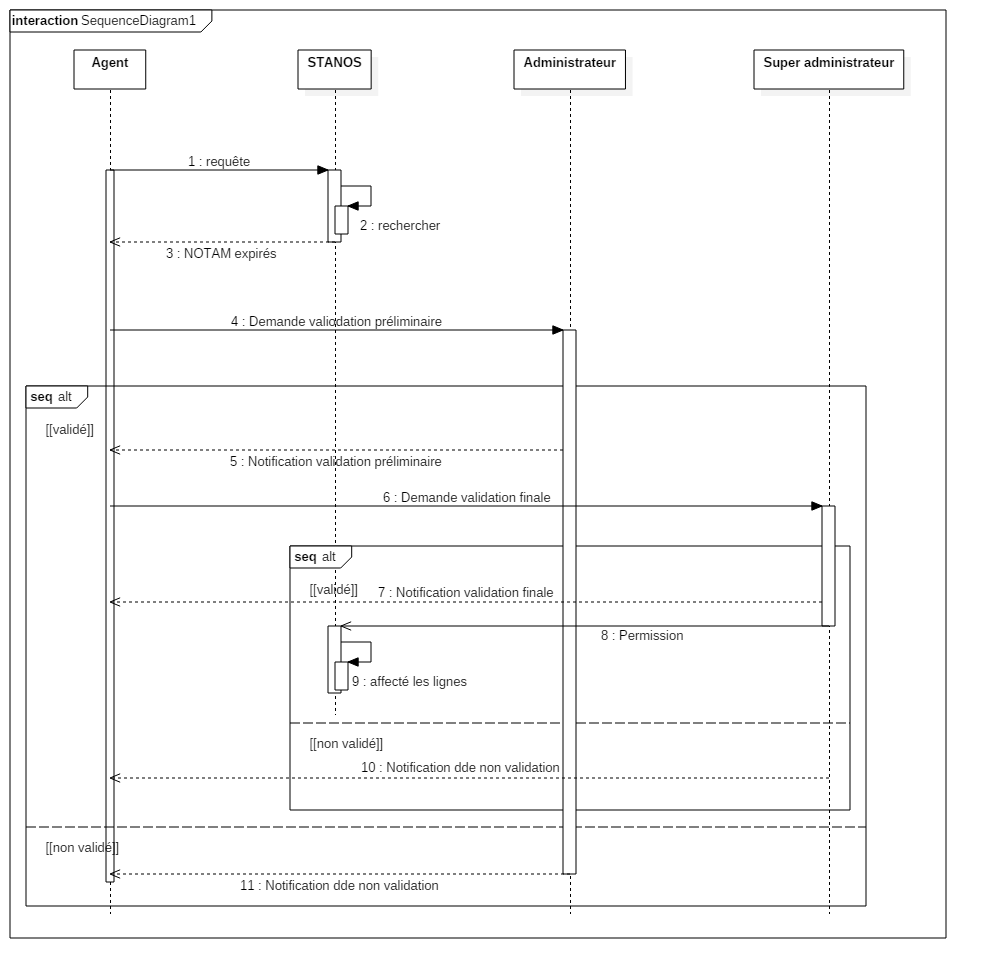
\includegraphics[width=17cm,height=18cm]{besoins/SequenceDiagram1.png}
\end{center}
%légende de l'image
\caption{Diagramme de séquences de l'opération connexion}
\end{figure}
\newpage
\section*{Conclusion}
A travers ce chapitre, nous avons présenté notre conception proposée pour l’application. Nous avons fourni, dans un premier temps, une conception globale à travers un schéma général décrivant l’organisation de notre application. Par la suite, nous avons détaillé la conception à travers quelques diagrammes UML.\\
Après avoir détaillé la conception adoptée pour la réalisation de cette application, nous décrivons dans le chapitre suivant la phase de réalisation.

%\chapter{Réalisation}
La phase de réalisation est la phase opérationnelle de la création d’un système informatique.
Elle consiste à la concrétisation et la matérialisation de toutes les phases
d’analyse au niveau graphique et technique.  Dans ce chapitre, nous commençons par
une description de l’environnement matériel, logiciel et de programmation. Nous enchaînons
par une étude comparative afin de justifier le choix des technologies adoptées. Par la suite, 
nous présentons quelques interfaces des modules réalisés, afin d’illustrer leurs fonctionnalités
principales.

\section{Environnement de travail}

Nous décrivons dans cette section l’environnement matériel et logiciel adopté pour l’implémentation de notre application.

\subsection{Environnement matériel}

{\bf Station de travail 1 :}\\
Marque: PC portable HP\\
Processeur: Intel Core i7 CPU\\
Mémoire: 8,00GO de RAM\\
Type système d'exploitation : Windows 10.\\
~\\

{\bf Station de travail 2 :}\\
Marque: Serveur HP ProLiant DL380 G7 \\ 
Processeur: 2 x Intel Xeon E5450\\
Mémoire: 4,00Go de RAM\\
Type système d'exploitation : Windows Server 2008 R2.\\

\subsection{Environnement logiciel}
Tout le long de la phase de développement, nous nous sommes servies de l’environnement
logiciel suivant :\\
\begin{description}

{\bf \item Cloud9 IDE :} 
Cloud9 IDE est un environnement de développement intégré en ligne, publié en open source de la version 3.0. Il prend en charge des centaines de langages de programmation, y compris C, C ++, PHP, Ruby, Perl, Python, JavaScript avec Node.js et Go. Il permet aux développeurs pour commencer avec le codage immédiatement avec des espaces de travail pré-configurés, collaborer avec leurs pairs avec des fonctionnalités de codage de collaboration, et les caractéristiques de développement web comme la prévisualisation en direct et les tests de compatibilité du navigateur. [Langage promotionnel]
Il est écrit presque entièrement en JavaScript, et utilise Node.js sur le back-end. Le composant éditeur utilise Ace. En Juillet 2014, il utilise des conteneurs de Docker pour ses espaces de travail, et est hébergé sur Google Compute Engine.
{\bf \item SQL*Plus : }SQL*Plus est un utilitaire en ligne de commande d'Oracle qui permet aux utilisateurs d'exécuter interactivement des commandes SQL et PL/SQL. Décliné en plusieurs versions (graphique et web), il est principalement distribué avec le produit Oracle Database.
{\bf \item SublimeText : }
Sublime Text est un éditeur de texte générique codé en C++ et Python, disponible sur Windows, Mac et Linux. Le logiciel a été conçu tout d'abord comme une extension pour Vim, riche en fonctionnalités.
Depuis la version 2.0, sortie le 26 juin 2012, l'éditeur prend en charge 44 langages de programmation majeurs, tandis que des plugins sont souvent disponibles pour les langages plus rares.
{\bf \item StarUML : }
c'est un logiciel open-source cédé par son ancien éditeur sous licence GNU GPL, dédié aux plate-formes Windows, il est développé en Delphi. Ses principaux avantages
sont sa simplicité d’installation et de prise en main, et la possibilité de générer le squelette
des classes en langages Java, C++, ActionScript3.0. De plus, le logiciel a été conçu en prévoyant l’ajout de plugin supplémentaire afin de pouvoir être adapté simplement aux besoins évolutifs de ses utilisateurs. Enfin StarUML gère l’exportation des données au format XMI, le standard pour l’échange d’informations de métadonnées UML basé sur XML, ainsi que l’exportation au format jpg afin d’intégrer les diagrammes au sein des  documents.
{\bf \item Texmaker :}
c'est un logiciel libre destiné à l'édition de documents LaTeX et fonctionnant sur GNU/Linux, Mac OS X, Windows et OS/2. Il est développé en C++ à l'aide de la bibliothèque Qt.
Cet éditeur offre un lot de fonctionnalités : support complet de l'Unicode, coloration syntaxique, correction orthographique lors de la frappe, auto complétion, pliage/dépliage de code, snippets, support des expressions régulières, sélection rectangulaire, gestionnaire de session...
\end{description}
\subsection{Les choix techniques }
Nous discutons dans ce paragraphe les choix technologiques adoptés pour le développement.
\begin{description}
{\bf \item Laravel :}
 Laravel est un framework web open-source écrit en PHP respectant le principe modèle-vue-contrôleur et entièrement développé en programmation orientée objet. Laravel est distribué sous licence MIT, avec ses sources hébergées sur GitHub. Laravel, créé par Taylor Otwel, initie une nouvelle façon de concevoir un framework en utilisant ce qui existe de mieux pour chaque fonctionnalité\cite{cite2}.
{\bf \item Microsoft SQL Server :}
Microsoft SQL Server est un système de gestion de base de données (abrégé en SGBD) incorporant entre autres un SGBDR (SGBD relationnel ») développé et commercialisé par la société Microsoft. Il ne fonctionne que sous les OS Windows. En fait MS SQL Server est une suite composée de cinq services principaux :\\
Le moteur relationnel (OLTP) appelé SQL Server ;\\
Le moteur décisionnel (OLAP) appelé SSAS (SQL Server Analysis Services) incluant un moteur de stockage pour les cubes, des algorithmes de forage (data mining) et différents outils de BI (Business Intelligence) ;\\
Un ETL (Extract Transform and Load) appelé SSIS (SQL Server Integration Services) destiné à la mise en place de logiques de flux de données, notamment pour alimenter des entrepôts de données (data warehouse) ;\\
Un outil de génération d'état appelé SSRS (SQL Server Reporting Services) permettant de produire des rapports sous différentes formes et exploitant les ressources du moteur décisionnel (bases "resportServer...") à la fois pour y stocker les rapports mais aussi y cacher les données de ces derniers afin de faire du "warmup" ;\\
Un système de planification de travaux et de gestion d'alerte appelé Agent SQL qui utilise lui aussi les services du moteur SQL (base msdb).
{\bf \item Bootstrab :}
Bootstrap est une collection d'outils utile à la création de sites et d'applications web. C'est un ensemble qui contient des codes HTML et CSS, des formulaires, boutons, outils de navigation et autres éléments interactifs, ainsi que des extensions JavaScript en option. C'est l'un des projets les plus populaires sur la plate-forme de gestion de développement GitHub.
{\bf \item SQL :} SQL (sigle de Structured Query Language, en français langage de requête structurée) est un langage informatique normalisé servant à exploiter des bases de données relationnelles. La partie langage de manipulation des données de SQL permet de rechercher, d'ajouter, de modifier ou de supprimer des données dans les bases de données relationnelles. Outre le langage de manipulation des données, la partie langage de définition des données permet de créer et de modifier l'organisation des données dans la base de données, la partie langage de contrôle de transaction permet de commencer et de terminer des transactions, et la partie langage de contrôle des données permet d'autoriser ou d'interdire l'accès à certaines données à certaines personnes.
Créé en 1974, normalisé depuis 1986, le langage est reconnu par la grande majorité des systèmes de gestion de bases de données relationnelles (abrégé SGBDR) du marché.
\end{description}



\section{Aperçu sur le travail réalisé}
Dans cette partie, nous allons présenter quelques interfaces pour montrer les services offerts.
par notre application.
\subsection{Déroulement du projet}
Notre projet se déroule sur quatre phases principales:
\subsubsection{Phase études et préparations}
Cette phase commence par une réunion entre les représentants de la DNA (Aspect technique) et de la DCCR (Aspect opérationnel) ainsi que les représentants des sites distants. L'ordre du jours de cette réunion est le suivant:\\
\begin{itemize}
\item Présentation de la solution.\\
\item Planifier l'étude sécurité.\\
\item Rôle des différents acteurs. \\
\item Coordination entre le site centrale et les sites distants.\\
\end{itemize}
\subsubsection{Phase réalisation}
C'est la phase de réalisation se fait à travers la coordination entre les trois corps:\\

\textbf{Partie technique:} La mise en exécution de l'apurement de la base avec la documentation qui lui convient.\\

\textbf{Partie opérationnel:} Validation de la partie technique ( Apurement documentation).\\

\textbf{Partie distant:} D'après la validation des deux derniers on prévoie l'exploitation de l'apurement faite.\\

\subsubsection{Phase déploiement}
Elle consiste sur la mise en service de la base dans le coté distant après avoir réaliser l'apurement.\\

\subsubsection{Phase validation}
Cette phase c'est pour vérifier et optimiser notre travail. Enfin, il faut prévoir un PV de clôture de l'opération.
\subsection{Captures de l'exécution}

Pour ouvrir une session et commencer les différentes opérations sur la base de donné du STANOS, un exploitant doit se connecter tout d’abord. La page de connexion est illustrée par la figure 5.1.\\


\begin{figure}[!h]
\begin{center}
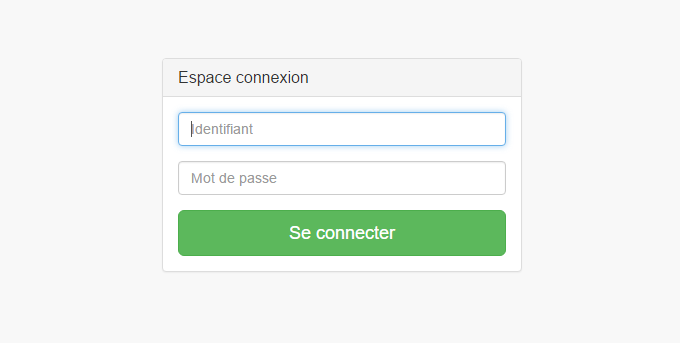
\includegraphics[width=9cm,height=4cm]{resultats/connexion.png}
\end{center}
%légende de l'image
\caption{Page de connexion}
\end{figure}
Le menu principal pour l’interface consacré au super administrateur contient quatre rubriques qui sont :
\begin{itemize}
\item Validation : cette rubrique contient toutes les notifications de validation qu’un super administrateur peut recevoir pour les valider. (Figure 5.2)\\
\item Gestion liste des utilisateurs : cette interface contient trois bouton ; un pour l’ajout d’un nouveau utilisateur, un deuxième pour modifier un compte déjà existant et un dernier pour supprimer un utilisateur. Cette interface est illustrée par la figure 5.3.\\
\item Message : contient un outil de communication entre les différents types d’exploitant (Figure 5.4).\\
\item Exception : cette rubrique est conçue pour gérer les opérations d’exception en cas d’urgence ou en cas d’enquête.\\
\end{itemize}

\begin{figure}[!h]
\begin{center}
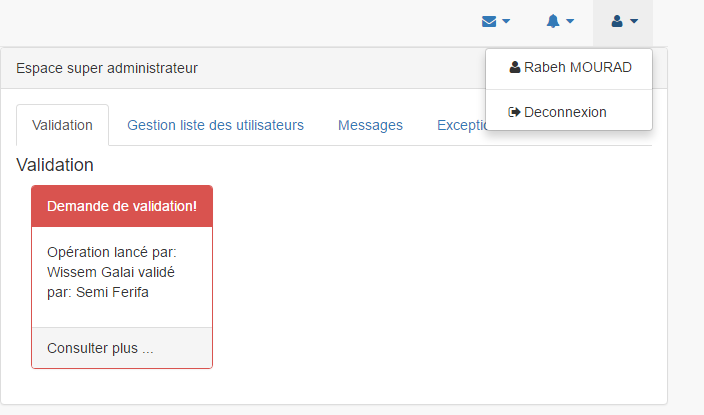
\includegraphics[width=10cm,height=4cm]{resultats/capture_validation.png}
\end{center}
%légende de l'image
\caption{Rubrique validation}
\end{figure}

\begin{figure}[!h]
\begin{center}
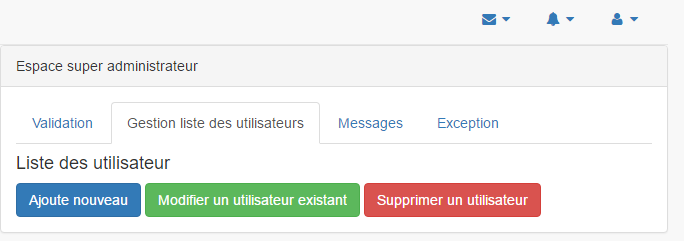
\includegraphics[width=10cm,height=6cm]{resultats/gestion.png}
\end{center}
%légende de l'image
\caption{Rubrique de gestion des utilisateurs}
\end{figure}

\begin{figure}[!h]
\begin{center}
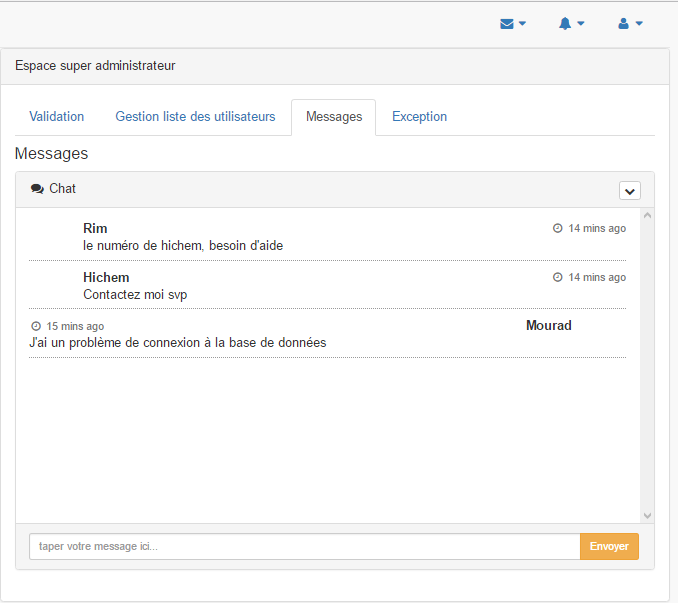
\includegraphics[width=10cm,height=6cm]{resultats/message.png}
\end{center}
%légende de l'image
\caption{Rubrique messages}
\end{figure}
\newpage
L’agent vérifie les NOTAM une à une pour les valider, cette validation se fait comme indiqué dans la figure 5.5. NB : le contenu de message dans la capture est un contenu à titre indicatif non pas le contenu réel des lignes de NOTAM.\\
\begin{figure}[!h]
\begin{center}
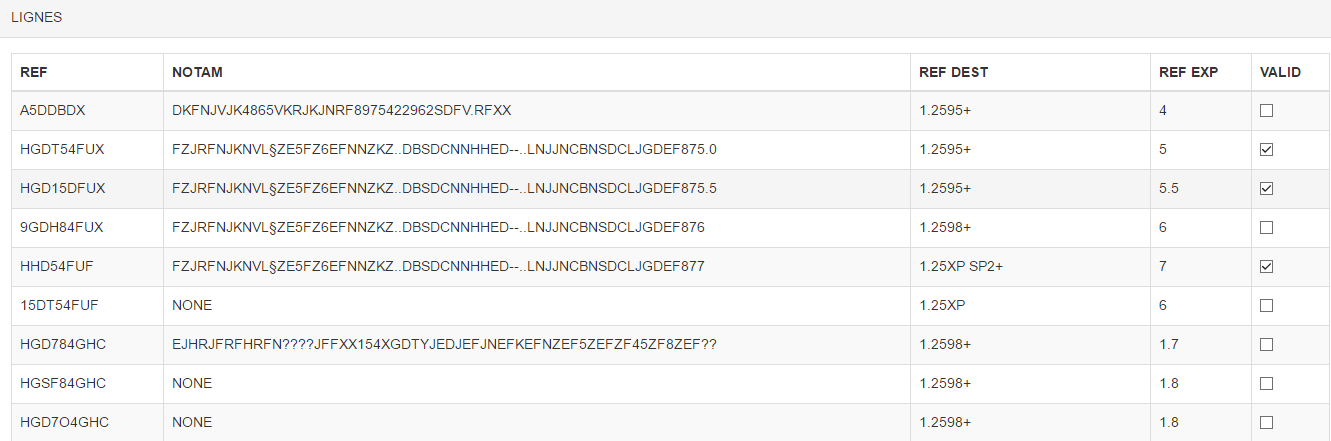
\includegraphics[width=15cm,height=6cm]{resultats/NOTAM.png}
\end{center}
%légende de l'image
\caption{Validation des lignes}
\end{figure}
\newpage
Après avoir validé les lignes à affecter, un agent configure la demande de validation puis la lance. Le traitement en cours de cette opération s’illustre par les figures 5.6, 5.7 et 5.8. \\
\begin{figure}[!h]
\begin{center}
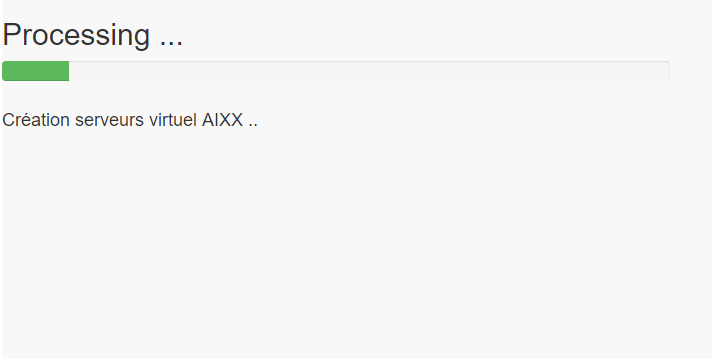
\includegraphics[width=10cm,height=6cm]{resultats/processing1.png}
\end{center}
%légende de l'image
\caption{Création du serveur virtuel AIXX}
\end{figure}

\begin{figure}[!h]
\begin{center}
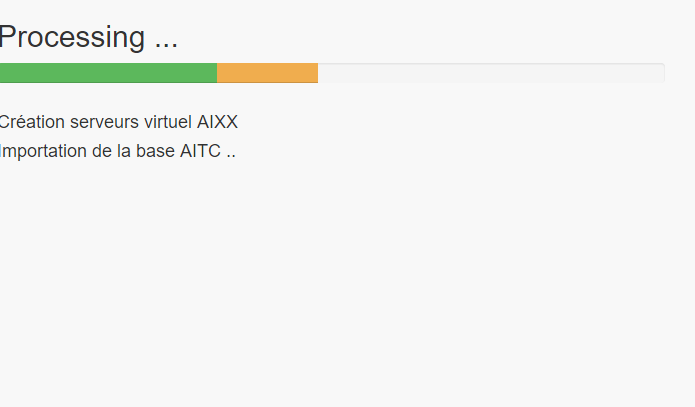
\includegraphics[width=10cm,height=6cm]{resultats/processing2.png}
\end{center}
%légende de l'image
\caption{Importation de la base AITC}
\end{figure}

\begin{figure}[!h]
\begin{center}
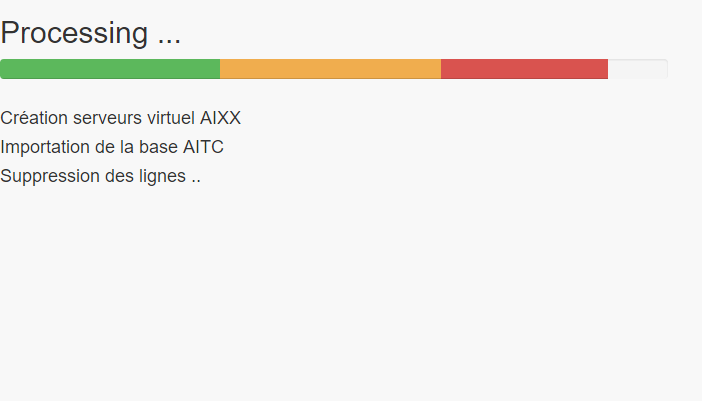
\includegraphics[width=10cm,height=6cm]{resultats/processing3.png}
\end{center}
%légende de l'image
\caption{Suppression des lignes NOTAM}
\end{figure}

\newpage


\section*{Conclusion}
Dans ce chapitre, nous avons présenté l’environnement et les technologies que nous avons
utilisées pour développer notre application. La première section de ce chapitre est réservée
à la présentation de l’environnement de travail utilisé. La deuxième section a été consacrée
à l’étude des choix techniques. La troisième section a exposé les principales interfaces réalisées
pour donner un aperçu sur le fonctionnement de l’application et le passage entre ses différentes
fenêtres.


%\chapter*{Conclusion Générale}
\addcontentsline{toc}{chapter}{Conclusion Générale}
%Rappel du context
Le travail élaboré dans le présent rapport a été effectué dans le cadre d’un projet développé au service DNA à l’OACA au cours du stage d’immersion en entreprise. Ce stage a pour but d’intégrer les élèves ingénieur  à l’ENSI dans le monde d’entreprise à la fin de la deuxième année. Il vise aussi de les préparer pour le projet de fin d’étude qu’ils auront à la fin de leur cursus universitaire.\\

Nous avons présenté dans ce rapport les différentes étapes menant à la conception et le développement d’une solution pour l’apurement de la base de données du système STANOS. \\

Dans le présent rapport, une étude afférente du sujet a été menée. Cette étude se décompose essentiellement en cinq chapitres. Dans le premier chapitre, nous avons présenté l’organisme d’accueil dans lequel nous avons effectué notre stage d’immersion en entreprise. On a présenté aussi dans ce chapitre le réseau RSFTA sur lequel porte notre projet de stage. Dans un deuxième chapitre, nous avons illustré l’état de l’art, nous avons aussi réalisé une étude de l’existant ainsi que le contexte du travail réalisé. Dans un troisième chapitre, nous avons spécifié les besoins qui doivent être précisé les différentes fonctionnalités du système et les services qui doivent les satisfaire. Dans le quatrième chapitre, nous avons déterminé la conception de l’application selon l’architecture MVC adoptée. Dans cette phase, nous avons présenté le diagramme de classes et le diagramme d’entité relation de la base de données du système développé. Pour le dernier chapitre intitulé « Réalisation », nous avons illustré l’aspect pratique de notre travail. En effet, nous avons défini l’environnement matériel et logiciel de notre réalisation. Dans une deuxième partie de ce chapitre, nous avons illustré dans des captures d’écran l’exécution de notre travail. \\

Tout au long de ce stage, nous avons essayé d’implémenter plusieurs fonctionnalités, tel que la gestion des rôles des utilisateurs, et la manipulation des bases de données en utilisant différentes technologies. Nous avons pu, alors, développer nos compétences techniques aussi bien que nos compétences soft au sein de l'entreprise (se présenter formellement, respect du temps, communiquer et se faire défendre ses idées, etc.. )\\

Enfin, nous pouvons conclure qu’il devrait toujours réfléchir à la contrainte de temps réel dans les systèmes de communication et savoir que la lenteur de transfert des messages peut mener à des situations critiques voir des catastrophes. C’est pour cette raison, il faut prendre en compte cette contrainte dans la conception de les bases de données des futurs systèmes pareils et prévoir une mise à jour automatique.  \\


%%Ne pas numéroter cette partie
\part*{Annexes}
%Rajouter la ligne "Annexes" dans le sommaire
\addcontentsline{toc}{part}{Annexes}

\chapter*{Annexe A}
\addcontentsline{toc}{chapter}{Annexe A}

%changer le format des sections, subsections pour apparaittre sans le num de chapitre
\makeatletter
\renewcommand{\thesection}{\@arabic\c@section}
\makeatother

%recommencer la numérotation des section à "1"
\setcounter{section}{0}

Autre que le projet développé au sein de l’OACA (Office d’Aviation Civile et des Aéroports), notre tâche était aussi d’effectuer des opérations préventives pour maintenir  le système fonctionnel. Cette annexe est consacrée pour énumérer les opérations à faire pour le système ADAMS.
\section*{Ce qu’il faut savoir faire sur l’ADAMS}

\begin{itemize}
\item Arrêt et démarrage d’un PC et de l’application AFTN.\\
\item Dépannage d’une imprimante (réinstallation, bourrage, changement de ruban, …). \\
\item Basculement onduleur sur batterie et retour sur Secteur. \\
\item Méthode de réclamation FR/RNIS. \\
\item Test de continuité d’une ligne. \\
\item Contrôle de la ligne Frame Relay.\\
\item Contrôle de la ligne RNIS. \\
\item Interprétation des voyants  des Modem.\\
\end{itemize}

\section*{Tâches quotidiennes}
\begin{itemize}
\item Vérifier l’état général.  \\
\item Faire l’archivage des données sur un CDROM : Il y a 3 fichiers essentiels qu’il faut copier (archive-out, ms,  event). Il ya une copie virtuelle sur un pc (on ne copie pas directement du serveur ADAMS) dont on prend une copie avec un décalage de deux jours et après avoir copié ce CDROM on fait une autre copie sur le PC  backup.\\
\item Vérifier l’état général des onduleurs.\\
\item Vérifier le système Insight Manager (compte rendu sur l’état hard et soft).\\
\item Vérifier la synchronisation du TMCS (Technical maintenance control system) : faire la synchronisation du TMCS selon GMT.\\
\item Vérifier le serveur actif (tu-cc1 ou tu-cc2) : il s’agit d’une commande linux sur le PC  backup grâce à une application « putty.exe », on introduit le login et le mot de passe et la commande « CLUSTAT ». \\
\item Vérifier le routeur actif : vérification visuelle. \\
\item Vérifier la climatisation.\\
\item Vérifier les lignes RNIS: on tape la commande « telnet tu-rt1 » sur l’invite commande puis on tape « sh isdn active » qui affiche les lignes RNIS qui sont fonctionnelles.\\
\item Redémarrer les transcodeurs: il faut toujours les redémarrer quand ils sont à l’état bas.\\
\end{itemize}

\section*{Tâches hebdomadaires}
\begin{itemize}
\item Vérifier le remplissage des disques système: c’est une commande « df-k » qui  indique automatiquement la taille des disques.\\
\item Tester les lignes RNIS: qui consiste à désactiver le Frame Relay au niveau soft.\\
\item Redémarrer le PC TMCS.
\end{itemize}


\section*{Tâches mensuelles}
\begin{itemize}
\item Tester les onduleurs: La maintenance de l’onduleur s’effectue tous les trente jours, en coupant le secteur afin de vérifier son bon fonctionnement et pour tester l’état des batteries. \\
\item Mettre à jour l’antivirus.
\end{itemize}


\chapter*{Annexe B}
\addcontentsline{toc}{chapter}{Annexe B}

%recommencer la numérotation des section à "1"
\setcounter{section}{0}

Dans cette annexe, nous présentons les tâches préventives à effectuer pour le système de messages aéronautiques STANOS.


\section*{Ce qu’il savoir faire sur le STANOS}
\begin{itemize}
\item Arrêt et Démarrage d’un PC client /serveur et de l’application BIA (Bureau d’information aéronautique)  et Distribution.\\
\item Dépannage d’une imprimante (réinstallation, bourrage, changement de ruban, …). \\
\item Basculement Onduleur sur batterie et retour sur Secteur.\\
\item Méthode de réclamation Frame Relay.\\
\item Test de continuité d’une ligne. \\
\item Contrôle de la ligne FR.\\
\end{itemize}
\section*{Tâches quotidiennes}
\begin{itemize}
\item Vérifier l’état général. \\
\item Vérifier la disponibilité des équipements: il s’agit d’une vérification visuelle dans l’application « Gestion des équipements STANOS ».
\begin{figure}[!h]
\begin{center}
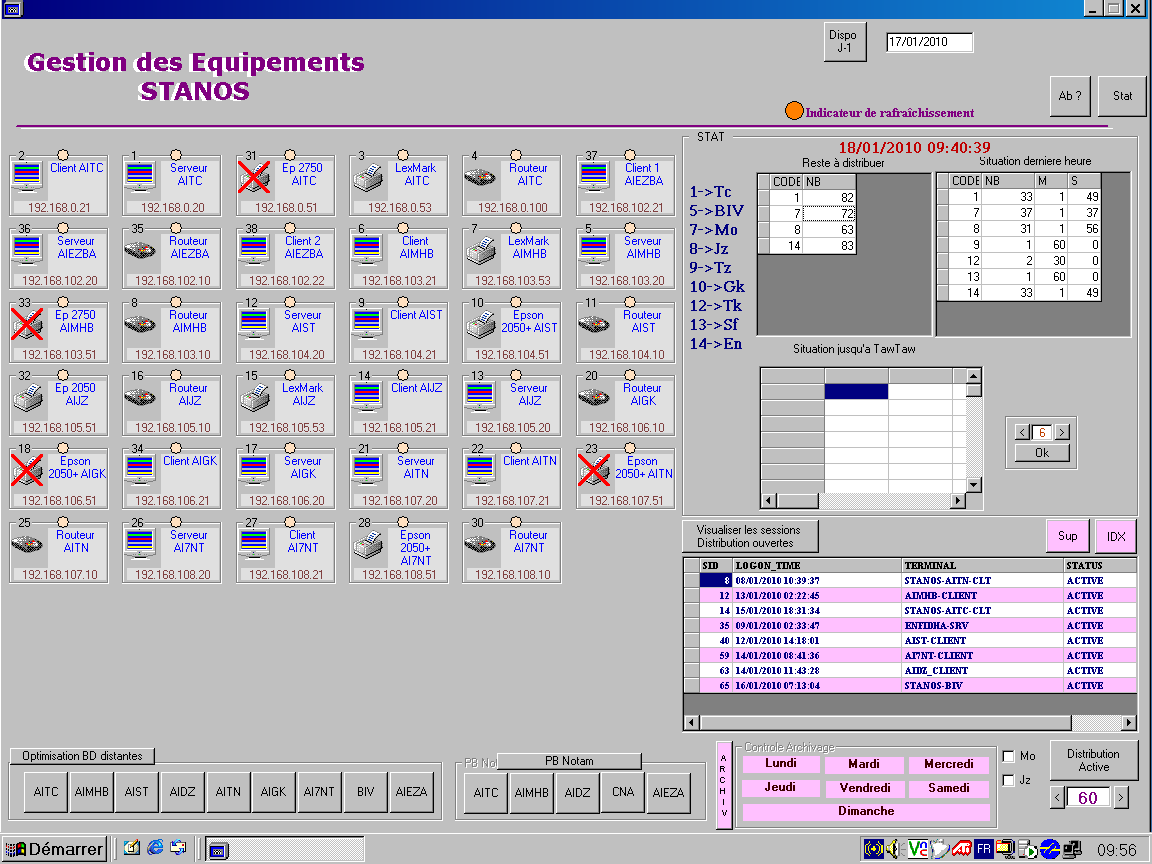
\includegraphics[width=10cm,height=7cm]{annexes/Gestion_des__quipements_STANOS.png}
\end{center}
%légende de l'image
\caption{Capture de l'application de gestion des équipements STANOS}
\end{figure}
\item Archivage de la base centrale sur le PC de supervision.\\
\item Optimisation de la distribution des messages par lancement d’une procédure de réindexassions et d’analyse des bases de données centrale et vérification des fichiers « log » qui contiennent un compte rendu de la dite procédure.\\
\item Archiver les données centrales + BIV sur une bande.
\item Vérifier le déroulement des Backups: archivage des données de chaque base  distante.\\
\item Vérifier la distribution des messages: taux de messages par minutes.\\
\item Vérifier l’état général des onduleurs.\\
\item Remplir la fiche GMAO.\\
\begin{figure}[!h]
\begin{center}
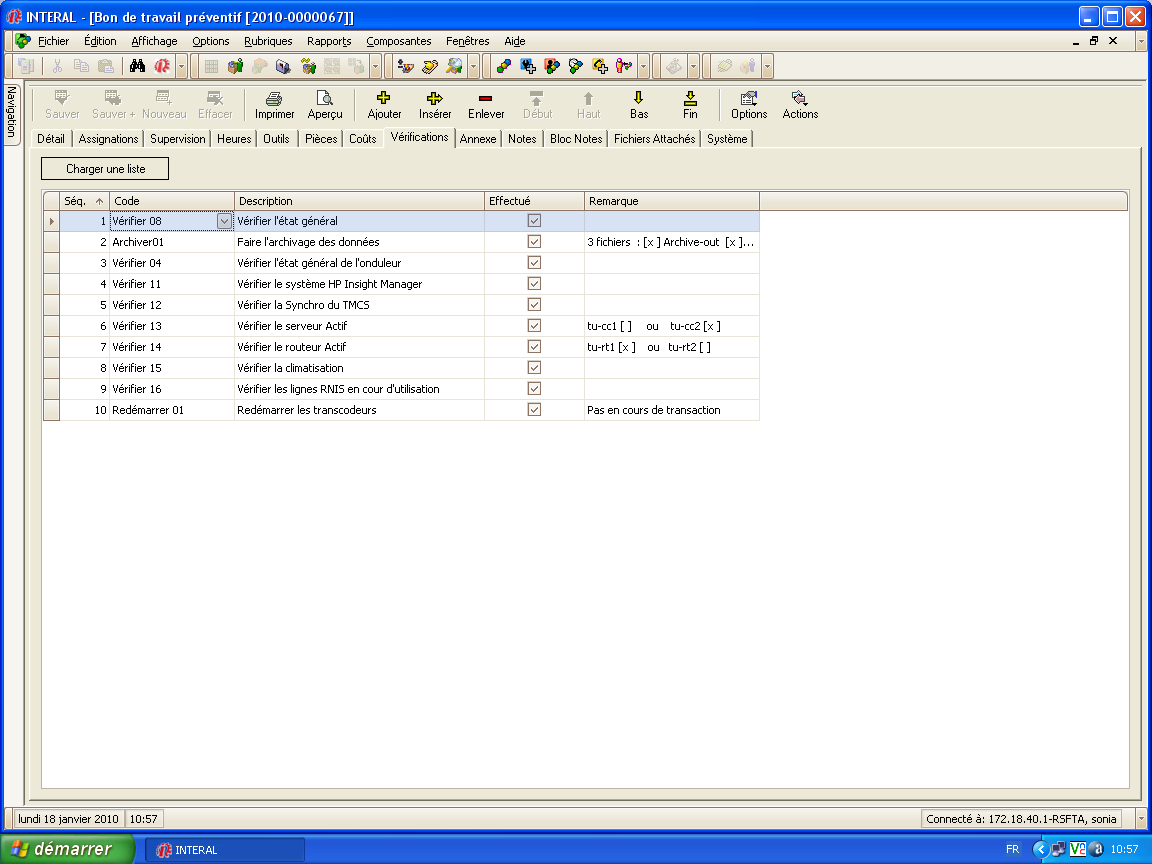
\includegraphics[width=10cm,height=7cm]{annexes/GMAO.png}
\end{center}
%légende de l'image
\caption{Capture de l'opération de remplissage de la fiche GMAO}
\end{figure}
\end{itemize}
\section*{Taches hebdomadaires}
\begin{itemize}
\item Optimisation de la distribution des messages par le lancement d’une procédure de réindexassions et d’analyse des bases de données distantes et vérification des fichiers « log » qui contiennent un compte rendu de la dite procédure.\\
\item Vérifier de l’espace libre disponible des disques système avec la commande \#df –k. (l’espace libre ne doit pas être inférieur à 20\% de l’espace total). \\
\item Synchronisation horaire entre les terminaux et la centrale (Manuellement).\\
\end{itemize}
\section*{Tâches mensuelles}
\begin{itemize}
\item Test des onduleurs: La maintenance de l’onduleur s’effectue tous les 30 jours, en coupant le secteur afin de vérifier son bon fonctionnement et pour tester la capacité des batteries. \\
\item Compactages des bases de données du module réception :
\begin{itemize}
\item Rendre esclave.\\
\item Arrêter l’application. \\
\item Désactiver le réseau. \\
\item Compacter la première base.\\
\item Redémarrer l’application.\\
\item Même procédure pour la deuxième base.\\
\end{itemize}
\end{itemize}

\begin{center}
\textbf{Remarque !}

\textit{Chaque tâche est planifiée dans le système GMAO (Gestion de maintenance assistée par ordinateur) et l'ingénieur est appelé à remplir le bon fonctionnement de la tâche réalisée.
 La validation est faite par le chef service.
}
\end{center}

\section*{Maintenances curatives}

\begin{table}[!h]
\begin{center}
\begin{tabular}{|p{8cm}|p{8cm}|}
  \hline
     \textbf{Problèmes} & \textbf{Solutions} \\
   \hline
   Pas de réception de trafic à SIDI AHMED &  -Remise à zéro du transcodeur de SIDI AHMED (coté CCR) -Demander aux techniciens de remettre à zéro le  transcodeur (coté SIDI AHMED) -Redémarrer le transcodeur de SIDI AHMED       -Relancer l’application ‘’IAT’’ -Vérifier que le test du transcodeur est bien reçu  \\ \hline
Panne de l’ATIS d’ENFIDHA & Contacter le technicien d’ENFIDHA ; problème reconnu par le fournisseur. \\ \hline
Faute de manipulation d’un onduleur au centre médical  & Déplacement sur place et réorganisation du branchement des équipements sur l’onduleur \\ \hline
Au cours du test de l’onduleur de STANOS on remarquer que l’autonomie batterie de cet onduleur est très faible. & Remplacement urgent par un autre onduleur plus performant. \\ \hline

  \end{tabular}
\end{center}
\caption{Tableau récapitulatif des problèmes possibles et leurs solutions}
\end{table}

\newpage

%récupérer les citation avec "/footnotemark"
\nocite{*}

%choix du style de la biblio
\bibliographystyle{plain}
%inclusion de la biblio
%\bibliography{bibliographie.bib}
%voir wiki pour plus d'information sur la syntaxe des entrées d'une bibliographie

\end{document}